\documentclass[12pt]{extarticle}
\usepackage{geometry}
\geometry{
a4paper,
total={170mm,257mm},
left=20mm,
top=20mm,
headheight=12pt
}

\usepackage[parfill]{parskip} % Activate to begin paragraphs with an empty line rather than an indent
\usepackage{graphicx}
\usepackage{amsmath, amssymb, amsthm}
\usepackage[font=small,labelfont=bf]{caption, subcaption}
\usepackage{setspace}\onehalfspacing
\usepackage[loose,nice]{units}
\usepackage{array}
\usepackage[super]{nth}
\usepackage{graphicx}
\usepackage{float}
\usepackage{varioref}
\usepackage[unicode=true,colorlinks=true,urlcolor=blue,citecolor=black,linkcolor=black]{hyperref}
\usepackage{cleveref}
\usepackage{subcaption}
\usepackage{mathtools}
\usepackage[all]{nowidow}
\usepackage{wrapfig}
\usepackage{pdfpages}
\usepackage{authblk}

% unbreakable dashes
\usepackage[shortcuts]{extdash}
% footnotes
\renewcommand{\thefootnote}{\fnsymbol{footnote}}

% less space before sections 
% \titlespacing*{<command>}{<left>}{<before-sep>}{<after-sep>}
\usepackage{titlesec}
\titlespacing*{\section}
{0pt}{2ex plus 1ex minus .2ex}{2ex plus .2ex}
\titlespacing*{\subsection}
{0pt}{1ex plus 1ex minus .2ex}{1ex plus .2ex}
\titlespacing*{\paragraph}
{0pt}{1ex plus 1ex minus .2ex}{1ex plus .2ex}

%SetFonts
% newtxtext+newtxmath
\usepackage{newtxtext} %loads helv for ss, txtt for tt
\usepackage{amsmath}
\usepackage[bigdelims]{newtxmath}
\usepackage[T1]{fontenc}
\usepackage{textcomp}
%SetFonts

% line numbers
\usepackage[displaymath, mathlines]{lineno}
 \renewcommand\linenumberfont{\normalfont\small\sffamily}
\linenumbers
\modulolinenumbers[2]

% Supplementary
\newcommand{\beginsupplement}{%
      	\setcounter{table}{0}
        \renewcommand{\thetable}{S\arabic{table}}%
        \setcounter{figure}{0}
        \renewcommand{\thefigure}{S\arabic{figure}}%
}

% NatBib
%\usepackage[super,comma]{natbib}
\usepackage[round,colon,authoryear]{natbib}
%\use-package[numbers,super,sort&compress]{natbib}
\renewcommand{\bibsection}{}
%\renewcommand{\bibfont}{\small}

% math stuff
\DeclareMathOperator*{\E}{{\rm I\kern-.3em E}}
\newcommand*{\tr}{^\intercal}
\let\vec\mathbf
\newcommand{\matrx}[1]{{\left[ \stackrel{}{#1}\right]}}
\newcommand{\diag}[1]{\mbox{diag}\matrx{#1}}
\newcommand{\goesto}{\rightarrow}
\newcommand{\dspfrac}[2]{\frac{\displaystyle #1}{\displaystyle #2} }
\newtheorem{theorem}{Theorem}
\newtheorem{corollary}{Corollary}
\newtheorem{lemma}{Lemma}
\newtheorem{remark}{Remark}
\newtheorem{result}{Result}
\renewcommand\qedsymbol{} % no square at end of proof
\newcommand{\cl}{\mathbf{L}}
\newcommand{\cj}{\mathbf{J}}
\newcommand{\ci}{I}

% title page stuff
\title{Prestige as a Driving Force in Cultural Transmission}

\renewcommand\Affilfont{\small}
\author[1]{Saar Egozi}
\author[2,3,*]{Yoav Ram}
\affil[1]{School of Computer Science, Reichman University, Herzliya 4610101, Israel}
\affil[2]{School of Zoology, Faculty of Life Sciences, Tel Aviv University, Tel Aviv 6997801, Israel}
\affil[3]{Sagol School of Neuroscience, Tel Aviv University, Tel Aviv 6997801, Israel}
\affil[*]{Corresponding author: yoav@yoavram.com, ORCID 0000-0002-9653-4458}
 
\date{\today}


\begin{document}
\maketitle

\begin{abstract}
Copying role-models can be an efficient method for acquiring knowledge. A common bias when choosing a role-model to copy is success bias: copying whoever appears more successful. This bias depends on the performance of the role-model alone, with no other factors. We propose an additional bias that may be prevalent in cultural transmission: influence bias, in which role-model choice is affected by the number of individuals that have already copied each potential role-model. We combine success and influence bias together to a ``prestige bias'' and analyze its effects on cultural-evolutionary dynamics using mathematical analysis and stochastic simulations. We find analytic approximations to our stochastic model, facilitating further mathematical analysis and reducing the computational complexity of simulations. We validate these approximations using simulations, and demonstrate their robustness to model assumptions.
We also find approximations to the fixation probability and the fixation time of an invading advantageous cultural trait, in both constant and changing environments, which resemble Kimura's approximations for population-genetic models.
These approximations show that success bias effectively plays the part of natural selection, whereas influence bias effectively reduces the population size.	
It also accelerates the evolutionary dynamics, as can be expected in a \textit{rich-getting-richer} process.
Our model may provide a good description of cultural transmission, 
especially in human societies where social media is popular. 
Further work is needed to test if this model could predict various phenomena in cultural evolution when extended with the effects of selection and innovation.
\end{abstract}
\pagebreak

\section*{Introduction}

\paragraph{Cultural transmission.}
In cultural transmission, individuals transmit cultural traits (i.e., behavior, beliefs, norms) to one another, typically via learning and demonstrating \citep{transmissionVectorsBook}.
Examples for cultural traits in humans are behavioral patterns, such as personalities and habits, transmitted via both verbally and by observations \citep{cultural_traits}. 
Although cultural transmission is most common in humans, it is also observed in other animals such as chimpanzees \citep{chimpsPrestige, chimpsCopy}, dolphins and whales \citep{dolphins_whales}.
In elephants, \citet{elepahntsRepo} showed that once a matriarch is removed from the group, the group's survival instincts are inferior and that ``the possession of enhanced discriminatory abilities by the oldest individual [matriarch] in a group can influence the social knowledge of the group as a whole.''
By playing audio recordings of African elephants, they showed that groups with a matriarch recognize and react better to hostile or friendly calls than groups without a matriarch.
\citet{fliesPaper} showed that choice of oviposition site in fruit flies is culturally transmitted: inexperienced flies that spent some time with experienced flies chose the same type of oviposition site even without directly observing this behavior. How the information is transmitted is still an open question, but it has been suggested that flies may use olfactory cues like other animals, such as rodents and bees.

\paragraph{Direction of transmission.}
Similar to genetic transmission, culturally transmitted traits can be transmitted from parents to offspring, and their effects of can be physiological rather than behavioral.
For example, parents can "teach" their children to be strong or tall, within some biological limits, by instructing them to maintain a specific diet and engage in physical activity.
Contrary to genetic transmission, cultural transmission can be non-vertical, that is, traits may be transmitted via social learning from non-parental individuals, and even unrelated individuals such as teachers, leaders, media, or any stranger that interacts with the learning individual.
Thus, cultural transmission may combine vertical transmission, where parents transmit to their offspring; oblique transmission, where adults transmit traits to unrelated offspring; and horizontal transmission, where peers from the same age cohort transmit to one another. 
Vertical transmission is also possible in the opposite direction: parents may copy traits from their offspring \citep{transmissionVectorsBook,transmissionVectors}.

\paragraph{Transmission biases.}
In social learning, transmission biases cause a trait to have a disproportionate probability to be transmitted compared to its frequency in the population.
Although more common in cultural transmission, transmission biases do occur in genetic transmission. For example, \textit{wtf genes} in yeast bias their transmission to the gamete by secreting a long life-expectancy poison together with a short life-expectancy antidote, so that a gamete without the gene will perish because the poison will outlive the antidote \citep{wtfGene}.
Importantly, even when a trait is disfavored by natural selection, it may still spread in a population due to transmission biases that are strong enough to overcome selection \citep[Ch. 8 pg. 279]{evolutionBook}.
\citet{cooperation} show that cooperative behavior can evolve in an individual due to horizontal transmission bias even when there is no benefit to it, or when it benefits its competitors.

\paragraph{Success bias.}
\citet{strategiesPaper} have conducted a tournament between learning strategies. Each strategy defines when individuals observe and copy from others, and when they engage in individual learning, in which an individual learns a cultural trait on his own. The best strategies had a high frequency of social learning relative to individual learning, even when the transmission error was almost 50\%. From these results we understand that all the winning strategies were mostly based on success biased social learning, meaning it contributed more to the general success of the population than individual learning. However, all winning strategies included individual learning to some degree, implying that success-biased learning alone isn't the best way to advance, even when success is measured accurately.


\paragraph{Evaluating success.}
\citet[Ch. 5]{evolutionBook} suggest that the evaluation of success can be divided into three groups: \textit{direct bias}, \textit{indirect bias} and \textit{frequency-dependent bias}.
A direct bias occurs when a variation of a trait is more attractive than others, and is evaluated by \textit{directly} testing the variation of the trait.
For example, an individual observing a Ping-Pong match can attempt both of the observed paddle grips to determine which grip is better.
An indirect bias occurs when an individual uses the value of one trait to determine the attractiveness of another, so it \textit{indirectly} evaluates the attractiveness of the role-model.
For example, an observer may copy the paddle grip of the Ping-Pong player who scored more points in the match, thus indirectly evaluating the grip by the points scored.
A frequency-dependent bias occurs when an individual has a probability to copy a variant of the trait that higher or lower than trait's frequency among demonstrators. 
For example, when an individual is 80\% likely to copy the common paddle grip even when only 60\% of the population is using it, it is said to be frequency-biased, or in this case, conformist.
Frequency bias could be negative, i.e., non-conformist bias. 
Conformity and non-conformity are well-known biases in cultural transmission \citep{conformism}, and its effect on cultural evolution have been studied with both models \citep{conformity,anticonformity} and experiments \citep{negativeFrequency}.
 
\paragraph{Prestige.}
Prestige means having a good reputation or high esteem, therefore does not directly signify success (although it may imply it), making it an indirect bias.
Both \citet[Ch. 8]{evolutionBook} and \citet{complexityPaper} suggest that prestige biases are probably more common in humans than success biases.
\citet[Ch. 8]{evolutionBook} add that maladaptive traits may spread widely in a population if indirect biases are strong enough.
They suggest that such biases could lead to a runaway process caused by a cultural equivalent of sexual selection \citep{sexualSelectionBook}.
On the other hand, \citet{fijian_social_bias} suggest that prestige biases, over generations, can lead to cultural adaptations, and that although prestige can lead to maladaptive traits spreading in the population, it can also accelerate the spread of adaptive traits.
Prestige is often mentioned in the cultural-evolution literature, but seldom modeled.

\paragraph{Influence bias.}
Today, social media provides an easy way to estimate the social and cultural influence individuals have over others, and therefore may have an effect on decision making. Online social networks such as \textit{Facebook} or \textit{Instagram} are known to affect the influence of individuals \citep{social_influence,influence_analysis,social_media}, and specific marketing practices were invented to capitalize on this effect \citep{facebook_marketing}.
Here, we model such influence as an indirect bias in cultural transmission, in which the choice of a role-model depends on the choices made by other individuals that have already chosen a role-model. 
Other than its relative ease of evaluation, compared to the evaluation of the actual trait, choosing a role-model based on previous choices made may be advantageous on its own. % TODO rephrase
This bias depends on the state of a role-model rather than on its trait, in contrast to frequency biases such as conformity,% TODO cite doi 10.1111/j.1420-9101.2011.02236.x
 which depend on the frequency of a trait in the population or in a sample of role-models. 
 We define a model of cultural transmission with prestige bias that combines both success and influence biases, provide analytic approximations for this model, and analyze its dynamics.

%%%%%%%%%%%%%%%%%%%%%%%%%%%%%%%%%%%%%%%%%%
\section*{Models and Methods}

We begin with a continuous trait model with indirect bias suggested by \citet{evolutionBook}, develop an extension with influence bias, and then develop a model with a dichotomous trait.
We implemented our stochastic models and approximations, performed statistical analyses, and produced figures using Python \citep{python} with NumPy \citep{numpy} and Matplotlib \citep{mathplotlib}. 
 
Source code is available at \href{https://github.com/yoavram-lab/PrestigeBias}{https://github.com/yoavram-lab/PrestigeBias}.

\subsection*{Continuous trait}
We follow the model of \citet{evolutionBook}, assuming only oblique transmission of the trait and omitting the indirect trait in order to reduce model complexity. 
We consider a population of $N$ individuals, described by a single trait with a continuous value.
Each generation, $N$ naive individuals, or copiers, choose an individual from the previous generation, or role-models, from which they will copy their trait. Similar to a Wright–Fisher model, we assume non-overlapping generations such that the entire population is replaced in each generation.
The population at time $t$ can be described by $\vec{A}(t)=\big(A_{1}(t), \ldots, A_{N}(t)\big)$ where $A_{i}(t)$ is trait value of individual $i$ at time $t$. We assume the initial population is drawn from a standard normal distribution, $\vec{A}(0) \sim N(0,1)$ .
Cultural transmission is modeled by a function $F$ such that 
\begin{equation}\label{eq:transmission}
A_{i}(t+1) = F_i(\vec{A}(t)) \;.
\end{equation}

\paragraph{Success bias.}
\citet[Ch.8, p.247-249]{evolutionBook} describe a blended transmission algorithm by defining $F$ as a weighted average of the traits of all role-models, 
\begin{equation}\label{eq:boydF}
F_i(\vec{A}) = \sum_{j=1}^N G_{i,j}\cdot A_{i,j} \;, 
\end{equation}
where $G_{i,j}$ is the success bias of role-model $j$ in the eyes of copier $i$,
\begin{equation}\label{eq:boydG}
G_{i,j} = \frac{\beta(A_{i,j})}{\sum_{k=1}^{N} \beta(A_{i,k})} \;,
\end{equation}
$A_{i,j}$ is the absolute trait value copier $i$ estimates for role-model $j$ with some error $e_i \sim N(0,\eta^2)$,
\begin{equation}\label{eq:relativeTrait}
A_{i,j} = A_j + e_i,
\end{equation}
and $\beta(\cdot)$ is the bias function that quantifies the success bias of a role-model,
\begin{equation}\label{eq:success_bias}
\beta(A_{i,j}) = b \cdot \exp{\Big(-\frac{(A_{i,j} - \hat{A})^2}{2J}\Big)},
\end{equation} 
with $\hat{A}$ as the arbitrary optimal trait value, and $J$ and $b$ as parameters that control the bias strength.
Therefore, $G_{i,j}$ is a relative success score that copier $i$ assigns to role-model $j$, equivalent to relative fitness in evolutionary-genetic transmission models.

\citet{evolutionBook} note that the deterministic blended transmission algorithm they use has alternatives. We thus develop a similar stochastic model with transmission from a single random role-model. Instead of \cref{eq:boydF}, we define the transmission function $F$ as a random variable with its distribution given by 
\begin{equation}\label{eq:ourF}
\Pr\big(F_i(\vec{A}) = A_{j}\big) = G_{i,j} \;,
\end{equation}
such that $G_{i,j}$ gives the probability of copier $i$ to choose to copy the trait of role-model $j$.

\paragraph{Influence bias.}
Here we introduce a new element to the model.
We assume that in each generation, copiers choose their role-models one by one.
We denote $K_{i,j}$ as the number of copiers that chose role-model $j$ after copier $i$ chose a role-model. Thus, $i$ out of $N$ copiers already chose a role-model, $\sum_{j=1}^N{K_{i,j}} = i$, and there are $N-i$ copiers that have yet to choose a role-model.
The stochastic process of role-model choice, 
\begin{equation} \label{eq:process}
\big\{\vec{K}_i = (K_{i,1}, \ldots, K_{i,N}) \big\}_{i=1}^N \;,
\end{equation}
is described by the recurrence equation
\begin{equation} \label{eq:recurrence}
K_{i,j} = K_{i-1,j} + S_{i,j}, \quad i,j=1,2,\ldots,N \;,
\end{equation}
where $S_{i,j}=1$ if the $i$-th copier chose role-model~$j$ and 0 otherwise, and the initial state is $K_{0,j}=0$.

Following \cref{eq:ourF}, the probability that the $i$-th copier chose role-model $j$ is given by the prestige of role-model $j$ in the eyes of copier $i$,
\begin{equation}\label{eq:recPrestige}
Pr(S_{i,j}=1 \mid S_{1,j},S_{2,j},...,S_{i-1,j}) = G_{i,j} \;.
\end{equation}
The prestige $G_{i,j}$ of role-model~$j$ in the eyes of copier~$i$ is determined by the estimated biased trait value $\beta(A_{i,j})$ and the number of copiers that chose role-model $j$ before copier $i$, $K_{i-1,j}$, replacing \cref{eq:boydG} of \citet{evolutionBook} with
\begin{equation}\label{eq:prestige}
G_{i,j} = \frac{\alpha_{ij} \cdot \beta(A_{i,j}) + (1-\alpha_{ij}) \cdot K_{i-1,j}}{W_i} \;.
\end{equation}
Here, the bias weight $\alpha_{ij}$ is a characteristic of the interaction of role-model~$j$ with copier $i$, that determines the relative significance of success and influence within the role-model's overall prestige, in the eyes if the copier. The trait of role-model $j$ estimated by copier $i$, $A_{i,j}$, remains as in \cref{eq:relativeTrait}, and $W_i$ is a normalizing factor that sums the numerator over all role-models ($1\le j \le N)$ to ensure $\sum_{j=1}^{N}{G_{i,j}}=1$.



\subsection*{Dichotomous trait}
To allow for mathematical analysis of the model, we introduce a simplified version where the trait only has two phenotypes: the optimal phenotype $\hat{A}$ and the sub-optimal phenotype $A$. 
All role-models with the same phenotype will contribute to the probability of that phenotype to be transmitted, and thus influence is determined by the number of copiers that have already chosen a role-model with either phenotype.
In addition, we assume homogeneous $\alpha$ for simplicity and for easier mathematical analysis.
Therefore, the probability of the $i$-th copier to copy phenotype $A$ is
\begin{equation}\label{eq:binary-model}
G_{i,A} = \frac{(N-X)\alpha'\beta(A) + K_{i,A}}{i-1 + (N-X)\alpha'\beta(A) + X\alpha'\beta(\hat{A})} = \frac{(N-X)\alpha'\beta(A) + K_{i,A}}{i-1 + (N-X)\alpha'\beta(A) + \alpha'X}
\end{equation}
where $X$ is the number of role-models with trait $\hat{A}$ and $K_{i,A}$ is the number of copiers that already chose $A$ when copier $i$ chooses a role-model and $\alpha'$ is the odd ratio of the bias weight $\alpha'= \frac{\alpha}{1-\alpha}$.

We prove this equation later, based on the proof of the Dirichlet-Multinomial approximation.

Initially, we assume the population has a single individual with phenotype $\hat{A}$ and $N-1$ individuals with phenotype $A$. The rest of the details follow the continuous trait model.

%%%%%%%%%%%%%%%%%%%%%%%%%%%%%%%%%%%
\section*{Results}
\subsection*{Approximations}
Our model is defined by two nested stochastic processes. Change over multiple generations is described by the phenotype distribution at each generation, $\{\vec{A}(t)\}_t$. The transition from one generation to the next is described by the number of copiers each role-model has after $i$ copiers have chosen a role-model, $\{\vec{K}_i\}_{i=1}^N$.
We emphasize that the models are nested: $\vec{A}(t+1)$ can be computed from $\vec{A}(t)$ by evaluating $\vec{K}_{N}$. However, the former requires iterating over \cref{eq:recurrence,eq:recPrestige}. Thus, we sought to find an equivalent stochastic process that has the same joint distribution as $\vec{K}_{N}$. 
We found two such approximations, summarized here and explained in detail below. In both we assume either $\alpha_j$ is a trait of role-model $j$ only (contrary to $\alpha_{ij}$ that included the relation with copier $i$), or a completely homogeneous $\alpha$.
\begin{enumerate}
\item 
The number of copiers of a specific role-model at each step, $K_{i,j}$, follows the {\em generalized binomial distribution}~\citep{GBD} and therefore,
\begin{enumerate}\item the expected number of copiers of role-model~$j$ equals its prestige in the eyes of the first copier, multiplied by the total number of copiers, that is,
$\E[K_{N,j}] = N \cdot G_{1,j}$ if trait estimation error is uniform for all copiers ($e=e_i$ for $i=1, \ldots, N$).
\item the expected number of copiers of each role-model equals its relative biased trait value, similar to the role of relative fitness in population-genetic models, that is, $\E[K_{N,j}] = \beta(A_j+e) / \overline{\beta}$ if the bias weight is uniform for all role-models ($\alpha=\alpha_j$ for $j=1,\ldots,N$), where $\overline{\beta}=1/N \sum_{j=1}^{N}{\beta(A_j+e)}$ is the population mean estimated trait value. 
\end{enumerate}
\item The role-model choice process, $\{\vec{K}_{i}\}_{i=1}^{N}$, is equivalent to a {\em P\'{o}lya urn} model if trait estimation error is uniform for all copiers ($e=e_i$ for all $i=1, \ldots, N$), meaning there's no meaning for the order of copiers. 
Therefore, the number of copiers of all role-models, $\vec{K}_i = (K_{i,1}, \ldots, K_{i,N})$, follows a Dirichlet-Multinomial distribution,
$\vec{K}_i \sim \mathit{DM}\big(N, \vec{G}_1\big)$, where $\vec{G}_1 = (G_{1,1}, \ldots, G_{1,N})$ is the prestige vector of all role-models in the "eyes" of the first copier.
Note that here $G_{i,j}$ is only a function of the trait values $A_j$ and the bias weights $\alpha_j$, as the estimation error is uniform, meaning all copiers are identical.
\end{enumerate}


\subsection*{Generalized binomial distribution}
The generalized binomial distribution (GBD) emerges from a series of dependent Bernoulli trials (in contrast to the standard binomial distribution in which trials are independent) and is parameterized by $GBD(n, p, \theta)$ where $n$ is the number of trials, $p$ is the probability of success of the first trial, and $\theta$ is the correlation between trials ($\theta=0$ gives the standard binomial distribution).
\\

\begin{result}[GBD approximation]\label{res:GBD}
The number of copiers of role-model $j$ after $i$ copiers have chosen a role-model follows the GBD, $K_{i,j} \sim GBD(i,\alpha_i\cdot\beta(A_j+e))$ if $e_i=e$ for all role-models $i=1, \ldots, N$. 
\end{result}

\begin{proof}
We denote $Q_j(k,i)=P(K_{i,j} = k \mid K_{i-1,j})$ as the probability that exactly $k$ out of $i$ copiers choose role-model $j$ given $K_{i-1,j}$ our of $i-1$ copiers chose role-model $j$. 
Using conditional probability and \cref{eq:recurrence},
\begin{equation}\label{recursive}
Q_j(k,i) = P_j(S_{i,j}=1 | k-1,i-1) \cdot Q_j(k-1,i-1) + P_j(S_{i,j} =0 | k,i-1) \cdot Q_j(k,i-1),
\end{equation}
where $S_{i,j} =1 $ when the $i$-th copier chooses role-model $j$.
\Cref{recursive} is equivalent to eq.~(2.1) by \citet{GBD}, which completes the proof.
\end{proof}

\begin{corollary}
$\E[K_{N,j}] = N \cdot G_{1,j}$.
\end{corollary}

\begin{proof}
\citet[eq.~(2.3)]{GBD} show that 
$\E[k] = N \cdot Q_j(1,1)$ (modified from their notation).
$Q_j(1,1)$ is the initial probability to choose role-model $j$, before any role-model choices are made.
$Q_j(1,1) = G_{1,j}$ by definition, which completes the proof.
\end{proof}

\begin{corollary}\label{cor:GBD}
$\E[K_{Nj}] = \alpha_j \cdot \beta(A_j+e) / \overline{\alpha \cdot \beta(A+e)}$, where the averaging in the denominator is over the role-models index, $j$.
\end{corollary}

\begin{proof}
The initial prestige of role-model $j$ based on \cref{eq:prestige} is
\begin{equation}\label{eq:initial_prob}
G_{1,j} = \frac{\alpha_j\cdot\beta(A_j+e)}{\sum\limits_{m=1}^{N} \alpha_m\cdot\beta(A_m+e)} \;.
\end{equation}
The denominator of \cref{eq:initial_prob} can also be formulated as:
\begin{equation}\label{eq:denominator}
 \sum\limits_{m=1}^{N}\alpha_m\beta(A_m+e) = N \cdot \overline{\alpha \cdot \beta(A+e)} \;,
\end{equation}
where $\overline{\alpha\beta(A+e)}$ is the mean value of $\alpha_m\cdot\beta(A_m+e)$ for all $m$.
Using \cref{eq:denominator} and \textbf{Corollary 1} we get,
\begin{equation}
\E[K_{Nj}] = \alpha_j \cdot \beta(A_j+e) \bigg/ \overline{\alpha \cdot \beta(A+e)} \;,
\end{equation}
completing the proof.
\end{proof}

The special case where the bias weight is uniform for all role-models ($\alpha = \alpha_j$ for $j=1,\ldots, N$) is interesting, because we can evaluate the expected number of copiers using a linear equation
\begin{equation}
\E[K_{Nj}]= N\cdot\frac{\alpha\cdot\beta(A_j+e)}{\sum\limits_{m=1}^{N}\alpha\cdot\beta(A_m+e)} =\beta(A_j+e) \bigg/ \overline{\beta(A+e)} \;,
\end{equation}
where the only variable is $A_j+e$, because $\overline{\beta(A+e)}$ is the mean of the distribution we draw the trait values from, modified by some constant parameters of $\beta$.
We can then denote $L = 1/\overline{\beta(A+e)}$ and write
\begin{equation}\label{eq:linearEq}
\E[K_{Nj}] = L\cdot \beta(A_j+e) \;.
\end{equation}

\paragraph{Numerical validation.}
To validate our results we ran $1,000$ simulations of the full model, and compared the results with \cref{cor:GBD}.
We compare the distribution of number of copiers by plotting the histograms of both our simulations results and the expected values based on \cref{cor:GBD}.
We used the average of the $1,000$ simulations to eliminate drift errors, as can be seen in \cref{fig:GBD}.

\begin{figure}[h]
    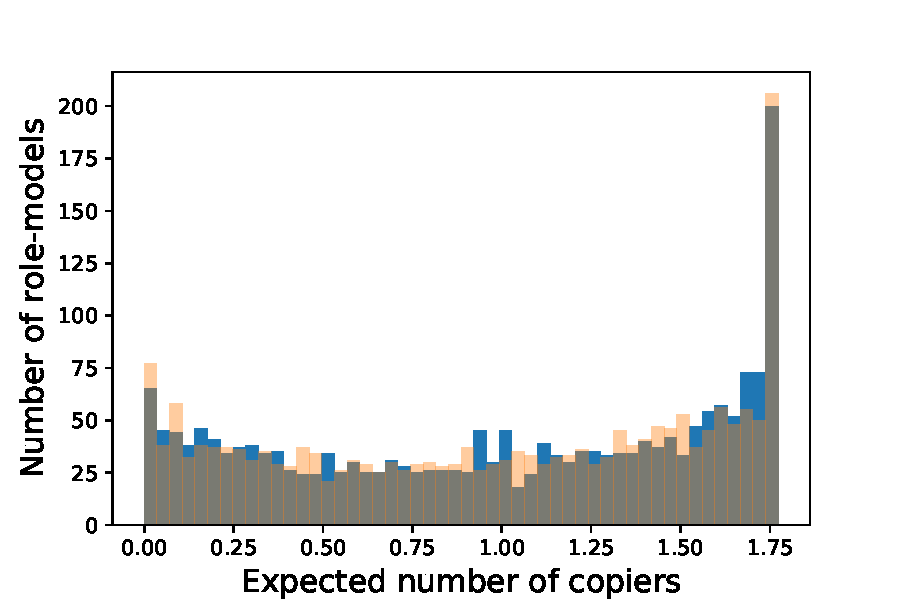
\includegraphics[width=\linewidth]{../figures/chi_square_stats/GBD_validation.pdf}
  \caption{
  \textbf{Numerical validation for the GBD approximation.}
  The approximation (orange) fits simulation results (blue) well when using 1,000 simulations for both models.
  Here, population size, $N=2,000$; bias weight, $\alpha=0.1$; idea phenotype value, $\hat{A}=1$; role-model traits $\vec{A} \sim N(0,1)$; success bias value, $\beta(A)=0.956$.}	
  \label{fig:GBD}
\end{figure}

Although basic, \cref{fig:GBD} shows good fit of the GBD approximation.
This validation is initial, and the more extensive validations we do on the Dirichlet-Multinomial approximation, because it is what we will use in our analysts.

\subsection*{Dirichlet-Multinomial distribution}

\paragraph{P\'{o}lya urn model.}
This stochastic process consists of $N$ draws from an urn with an initial amount of colored balls of $M$ colors. When a ball is drawn, it is then placed back in the urn together with an additional new ball of the same color.
Let $\vec{U_i} = \{u_{i,1},u_{i,2},...,u_{i,M}\}$  where $u_{i,j}$ is the number of balls of the $j$-th color in the urn after $i$ draws.
Let $S_{i,j}=1$ when drawing a $j$-colored ball on the $i$-th draw, and $0$ otherwise. The probability that $S_{i,j}=1$ given $\vec{U_{i-1}}$ is
\begin{equation}\label{eq:polya}
\begin{split}
P(S_{i,j} = 1 \mid \vec{U_{i-1}}) = 
\frac{u_{i-1,j}}{\sum\limits_{m=1}^{M} u_{i-1,m}} = 
\frac{o_j + w_{i-1,j}}{\sum\limits_{m=1}^{M} o_m + w_{i-1,m}} = 
\frac{o_j + w_{i-1,j}}{i-1 + \sum\limits_{m=1}^{M} o_m} \;,
\end{split}
\end{equation}
where $o_j$ is the initial number of balls of the color $j$ in the urn, and $w_{i,j}$ is the cumulative number of new balls that were added to the urn after $i$ draws of the color $j$.
\\

\begin{result}[P{\'{o}}lya urn model]\label{result:polya}
The role-model choice process, $\big\{\vec{K}_i\big\}_{i=1}^N$, is equivalent to a \textit{P\'{o}lya urn model} if both trait estimation error and bias weight are uniform in the population, $e=e_j$ and $\alpha=\alpha_j$ for all $j=1,\ldots,N$.
\end{result}

\begin{proof} 
Denote $\alpha'=\frac{\alpha}{1-\alpha}$ as the bias weight ratio, and $A'_j=A_j+e$. From \cref{eq:prestige} and because $\sum_{j=1}^{N}{K_{i,j}}=i$, we have
\begin{equation}\label{eq:copier_choose}
G_{i,j} = 
\frac{\alpha'\beta(A'_j) + K_{i-1,j}}{\sum\limits_{m=1}^{N} \alpha'\beta(A'_m) + K_{i-1,m}}
 =\frac{\alpha'\beta(A'_j) + K_{i-1,j}}{i-1 + \sum\limits_{m=1}^{N}\alpha'\beta(A'_m)} \;.
\end{equation}
Substituting $M=N$, $o_j = \alpha'\beta(A'_j)$, and $w_{i,j} = K_{i,j}$ in \cref{eq:polya} gives \cref{eq:copier_choose}, thus completing the proof.
\end{proof} 

\citet[section 2]{dirichlet} prove that the proportion of different colored balls in a \textit{P\'{o}lya urn model} converges to the Dirichlet distribution as the number of draws approaches infinity, based on the \textit{Martingale Convergence Theorem} \citep{martingaleBook}.
We therefore have an approximation for the relative prestige each role-model has when evaluated by copiers. Thus, choosing the role-models for all copiers is equivalent to drawing from a Multinomial distribution where the parameters are the modified weights from a Dirichlet distribution and we have the following corollary.
\\

\begin{corollary}\label{cor:dirichlet}
The number of copiers of each role-model follows a Dirichlet-Multinomial distribution, $\vec{K_i} \sim \textit{DM}(N,\vec{G_1})$, under the conditions of \Cref{result:polya}.
\end{corollary}

\paragraph{Numerical validation.}
To validate our analytical result (\cref{cor:dirichlet}) and test its sensitivity to the assumptions ($e_i=e$ and $\alpha_i=\alpha$ for $i=1,\ldots,N$) we compare it to results of stochastic simulations of the full model.
First, we computed an observed distribution of the number of copiers from the average empirical distribution of multiple simulations.
We then compared this observed distribution with the expected theoretical DM distribution as can be seen in \cref{fig:DM_validation} (a). The difference in distributions was not perceived when plotting both distributions on the same figure, so we used the difference instead. The maximum difference is 0.5 role-models, which indicate a very good fit.
In addition, we tested the likelihood of the observed data to be drawn from the DM distribution, against a shuffle of the parameters vector of the DM distribution itself, as seen in \cref{fig:DM_validation} (b). We see that the negative log likelihood of the observed data is much higher than any other shuffled version of the parameters vector, supporting our approximation more.


\begin{figure}[h]
    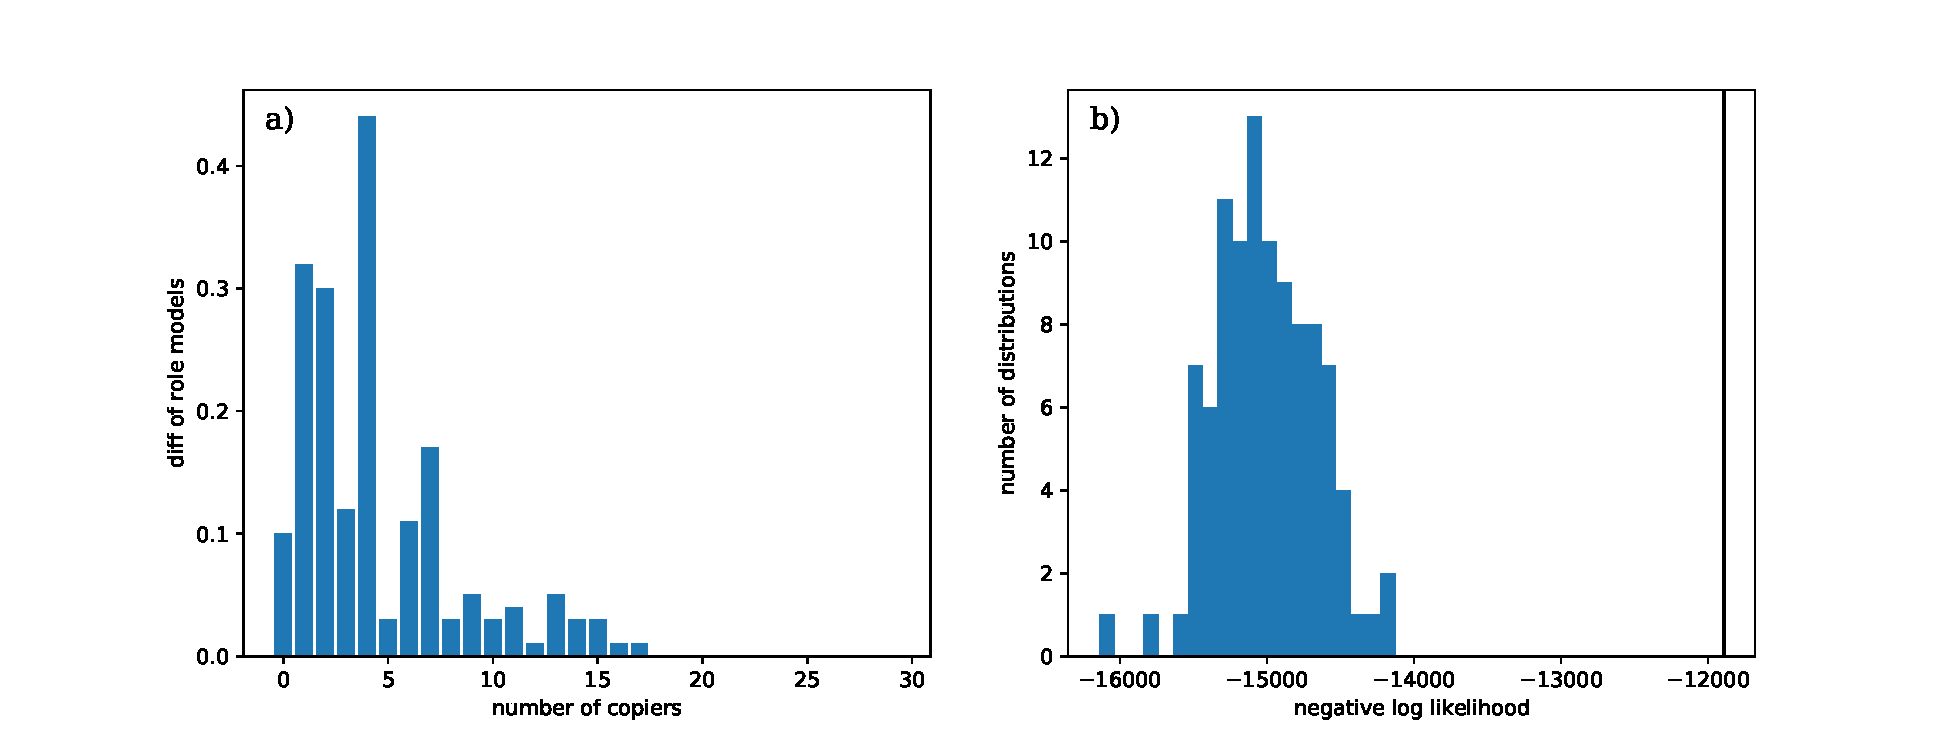
\includegraphics[width=\linewidth]{../figures/chi_square_stats/DM_validation.pdf}
  \caption{
  \textbf{Goodness of fit of Dirichlet-Multinomial approximation to the model.}
  The difference between the DM approximation distribution to observed model distribution (a) is very small, with the highest difference at 0.5 role-models.
  The optimal negative log likelihood (b) is given when using the DM approximation (black vertical line), and is much better when compared to a shuffled vector of the DM distribution (blue bars).
  Here, population size, $N=100$; number of distributions averaged, $m=100$; phenotype values, $\hat{A}=1$, $A \sim N(0,1)$; homogeneous success bias weight, $\alpha=0.5$.}	
  \label{fig:DM_validation}
\end{figure}


Next, we examined the fixation probability and fixation time of an advantageous phenotype $\hat{A}$ when invading a population of phenotype $A$ and compared results from the full model and the DM approximation.
We find that the number of simulations needed to sufficiently approximate our model with the DM approximation is roughly $1,000$ (\Cref{fig:num_sims}).
Next, we examined the robustness of the DM approximation to relaxing the approximation assumptions.
First, we relaxed our assumption of no estimation error $e$.
Estimation error in the original model was drawn from a normal distribution, and added to the trait value before evaluation of the bias ($A_{ij} = A_j + e_i$).
When estimation error is applied, we sample $J_i$ for each copier $i$ from a normal distribution with varying scale (variance).
Even when the standard deviation is $0.1$, the fixation probability and time is similar~(\cref{fig:hetro_error}). 
We also relaxed our assumption of a uniform bias weight $\alpha$ (i.e., $\alpha_i=\alpha$). We allowed $\alpha$ to vary in the population, drawing $\alpha_j$ for each role-model $j$ from a normal distribution such that $\alpha_j \sim N(0.5,x)$ where $x \in [10^{-7},10^{-1}]$. 
We found again that results of the DM approximation are similar to those from stochastic simulations of the full model~(\cref{fig:hetro_alpha}).



\begin{figure}[h]
    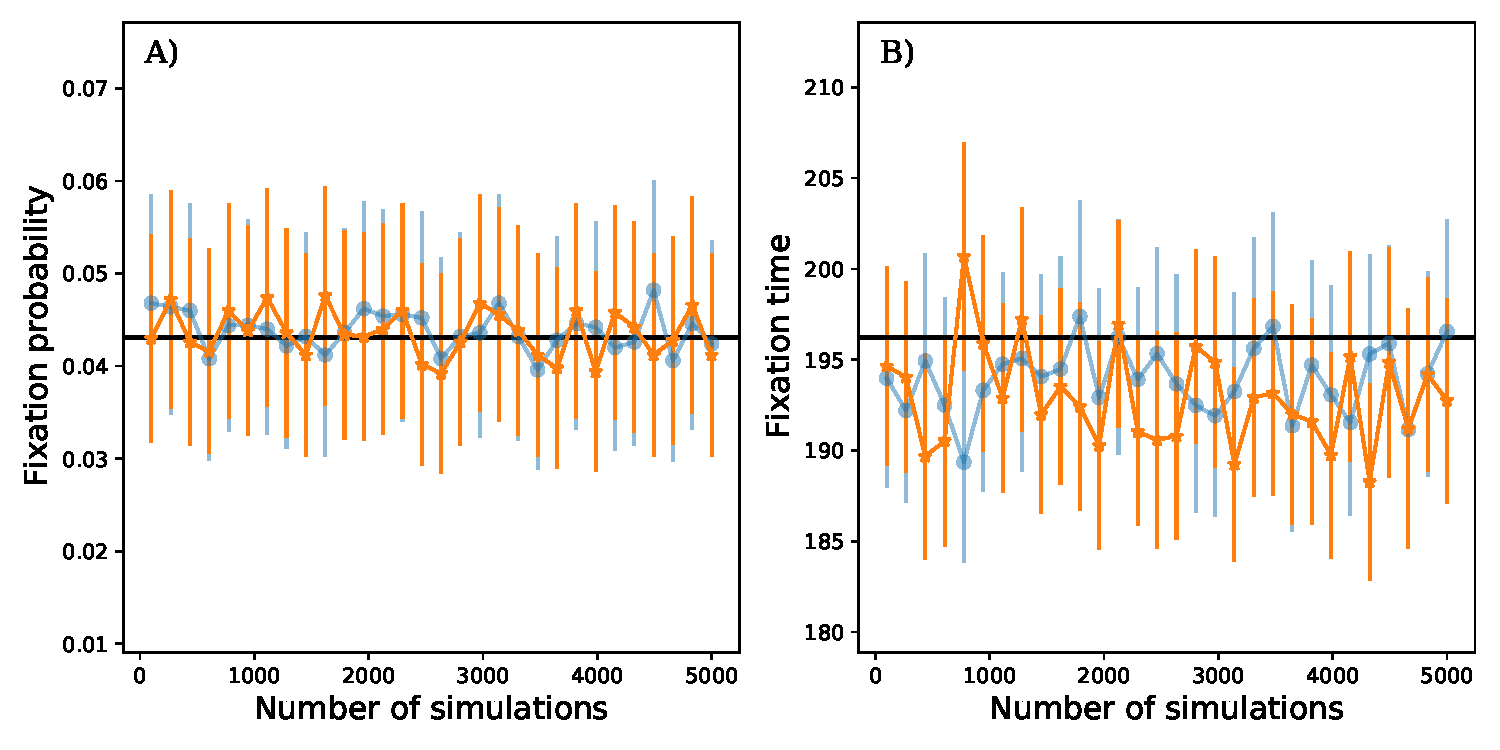
\includegraphics[width=\linewidth]{../figures/binary/num_sims.pdf}
  \caption{
  \textbf{Minimum number of simulations required to get a good approximation.}
  The approximation (orange) fits simulation results (blue) well when using 1,000 simulations for both models. The approximated value (black) is given by equation \cref{eq:kimura_p}.
  Markers for average value across simulations, error bars for 95\% confidence interval.
  Here, population size, $N=1000$; bias weight, $\alpha=0.5$; phenotype values, $\hat{A}=1$, $A=0.7$; success bias value, $\beta(A)=0.956$.}	
  \label{fig:num_sims}
\end{figure}


\begin{figure}
    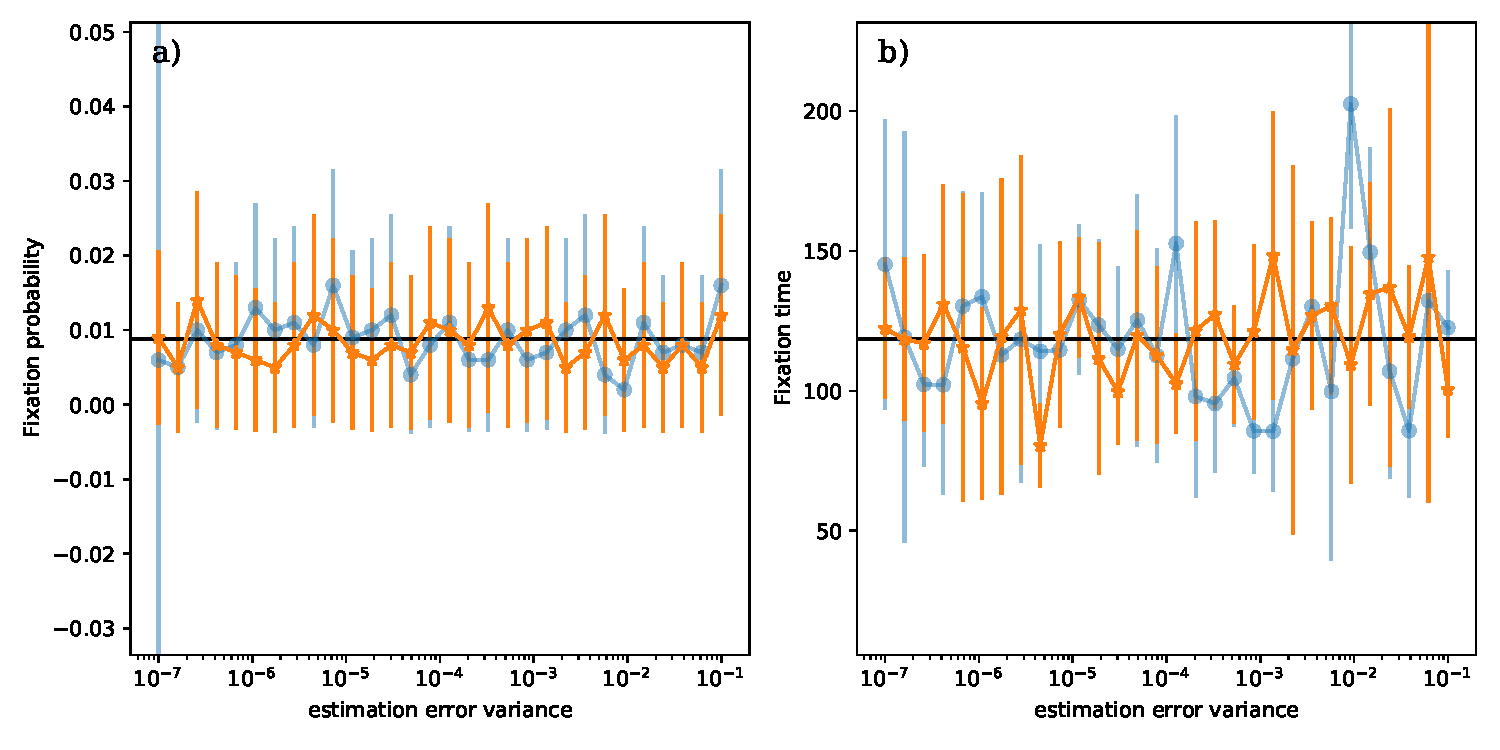
\includegraphics[width=\linewidth]{../figures/binary/full_vs_dm_mutation.pdf}
  \caption{
  \textbf{Robustness of DM approximations to inclusion of estimation error.} Both the DM approximation (orange) and Kimura's equation (black line) fit the stochastic simulations (blue) well even with a high estimation error rate. Markers for average across simulations, error bars for 95\% confidence intervals.
  5,000 simulations per data point; population size, $N=1000$; bias weight, $\alpha=0.1$; phenotype values, $\hat{A}=1$,$A=0.7$; bias strength parameter $J\sim N(1,x^2)$ where $x \in [10^{-7},10^{-1}]$.
  }	
  \label{fig:hetro_error}
\end{figure}


\begin{figure}
    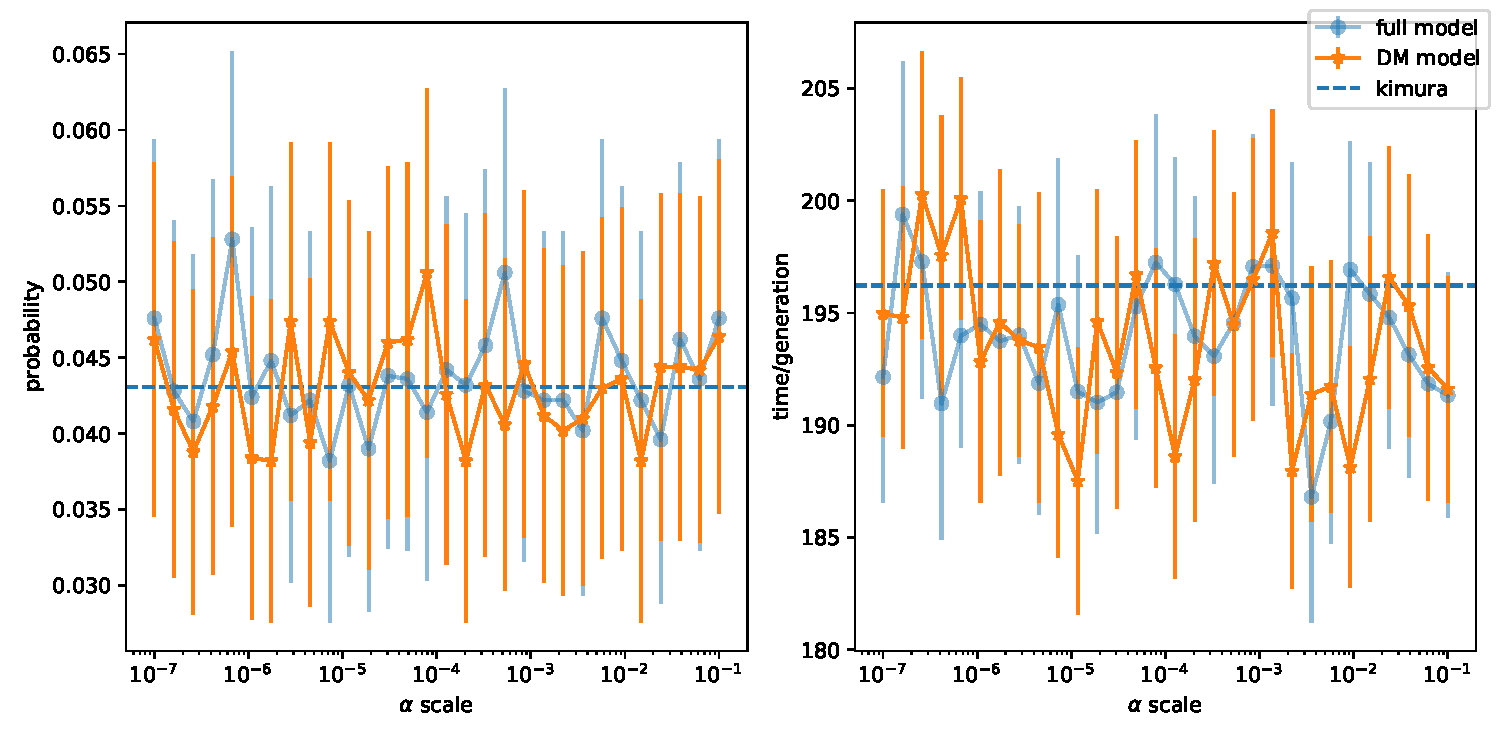
\includegraphics[width=\linewidth]{../figures/binary/full_vs_dm_changing_alpha.pdf}
   \caption{\textbf{Robustness of DM approximations to variation in the bias weight $\alpha$.} 
   Both the DM approximation (orange) and Kimura's equation (black line) fit the stochastic simulations (blue) well even with a high variation in success bias weight.Markers for average across $5,000$ simulations, error bars are 95\% confidence intervals.
  Here, population size, $N=1000$; success bias weight normally distributed, $\alpha\sim N(0.5,x^2)$; phenotype values ,$\hat{A}=1$,$A=0.7$; success bias value, $\beta(A)=0.956$.}	
  \label{fig:hetro_alpha}
\end{figure}


%%%%%%%%%%%%%%%%%%%%%%%%%%%%%%%%%%%%%%%%%%%
\subsection*{Fixation probability and time}

After finding that the DM distribution is a good approximation of the (within-generations) role-model choice process, we turn our attention to the (between-generations) evolutionary dynamics.
We focus on the fixation probability and fixation time of an advantageous phenotype, similar to analyses in population-genetic models \citep{kimura,kimura_average,otto_fixation}.

We are mainly interested in the effect of the bias weight ($\alpha$), which determines the relative effects of success and influence on prestige bias.
For simplicity, we do not include estimation error in this analysis.
As shown above, transmission in our model is approximately DM distributed with the parameters $\sim DM(\alpha'X,(N-X)\alpha'\beta(A))$ based on \cref{cor:dirichlet} and \cref{eq:copier_choose}.


\begin{remark}[Effective selection coefficient]
In population genetics a selection coefficient is a measure of differences in relative fitness. Selection coefficients are central to the quantitative description of evolution, since fitness differences determine the change in genotype frequencies attributable to selection.
Effective selection coefficient is the equivalent in a model to the selection coefficient in a Wright-Fisher model.
\end{remark}

\begin{result}[Effective selection coefficient]\label{res:selection_coef}
$1-\beta(A)$ is equivalent to the selection coefficient $s$ in the diffusion-equation approximation of the a classic Wright-Fisher model that approximate the fixation probability and fixation time of an advantageous allele.
\end{result}

\begin{proof}
Let $x$ be the frequency of type $\hat{A}$ in the population with $N$ individuals. Let $X$ be the number of individuals of type $\hat{A}$ so $x=X/N$. $X'$ is the number of individuals with $\hat{A}$ in the next generation and $x'$ their frequency.
By definition $\beta(\hat{A})=1$, and for simplicity we'll denote $\beta(A)=\beta$ ($\beta<1$).

The expected number of individuals of a DM distribution is:
\begin{equation}
E[X'] = N  \frac{\alpha_1}{\alpha_1+\alpha_2},
\end{equation}
where $\alpha_1 = \alpha' X$ and $\alpha_2 = \alpha'(N-X)\beta$, from  \cref{eq:binary-model}.
We want to use frequencies instead of quantities to follow Durret's process so:
\begin{equation}
E[x'] = E[\frac{X'}{N}] = \frac{1}{N}E[X']
\end{equation}
Putting it together we get:
\begin{equation}
\begin{split}
E[x'] &= \frac{1}{N}N\frac{\alpha' xN}{\alpha' xN + \alpha' N (1-x)\beta}\\
	 &= \frac{x}{x + (1-x)\beta}
\end{split}
\end{equation}

which is identical to the equation in the top of page 253, chap 7.2 in \citet{durret}. We therefore use the same approximation and say that:
\begin{equation}
\begin{split}
E[x'] =& \frac{x}{x + (1-x)\beta} = \frac{x}{x + (1-x)(1-s)} =\\
 &= x + x(1-x)s + o(s)\\
  &= x + x(1-x)(1-\beta) + o(1-\beta)
\end{split}
\end{equation}

By definition, $x$ is constant, so $E[x] = x$. We continue to calculate $E[x'-x]$:
\begin{equation}\label{eq:expec_freq}
E[x'-x] = E[x'] - E[x] = x(1-x)(1-\beta) + o(1-\beta)
\end{equation}
where when substituting $1-\beta$ with $s$, we get the same result as \citet{durret} which is the desired result.
\end{proof}

\begin{remark}
The effective size of a population, $N_e$, determines the rate of change in the composition of a population caused by genetic drift, which is the random sampling of genetic variants in a finite population. Ne is crucial in determining the level of variability in a population, and the effectiveness of selection relative to drift.
\end{remark}

\begin{result}[Effective population size]\label{res:effective_population}
$N_e=\alpha N + (1-\alpha)$, where $Ne$ is the effective population size of the binary model.
\end{result}

\begin{proof}
The variance of a DM distribution is:
\begin{equation}
V(X') = N\frac{\alpha_1}{\alpha_1+\alpha_2}(1-\frac{\alpha_1}{\alpha_1+\alpha_2})
(\frac{N + \alpha_1+\alpha_2}{1+\alpha_1+\alpha_2})
\end{equation}
And again, we want to use frequencies so:
\begin{equation}
V(\frac{X'}{N}) = \frac{1}{N^2}V(x')
\end{equation}

Putting it together with our model's notations:
\begin{equation}
V(x') = \frac{1}{N^2}N\frac{x}{x+(1-x)\beta}(1-\frac{x}{x+(1-x)\beta})
(\frac{N + \alpha' xN + \alpha' N(1-x)\beta}{1 + \alpha' xN + \alpha' N(1-x)\beta}) 
\end{equation}

Like Durrett, we'll use the zero order of the approximation when $\beta\approx1$,so:
\begin{equation}
\frac{x}{x + (1-x)\beta} \approx x
\end{equation}
and we also use $\beta\approx1$ for the entire variance expression and get:
\begin{equation}
\begin{split}
V(x') & \approx  \frac{1}{N} x(1-x)
(\frac{N + \alpha' xN + \alpha' N - \alpha' xN}{1 + \alpha' xN + \alpha' N - \alpha' xN})\\
&=  x(1-x)(\frac{1 + \alpha'}{1 + \alpha' N}) 
\end{split}
\end{equation}

Again following Durrett we want to calculate:
\begin{equation}\label{eq:var_diff_durret}
V(x'-x) = V(x') - V(x) \approx  x(1-x)(\frac{1 + \alpha'}{1 + \alpha' N})
\end{equation}
because $x$ is a constant so $V(x) = 0$

In our model, $\alpha'$ is the odds ratio of a parameter we called "bias weight", denoted in our model as $\alpha$, so:
\begin{equation}\label{eq:success_ratio}
\alpha' = \frac{\alpha}{1-\alpha}
\end{equation}

Combining \cref{eq:var_diff_durret} and \cref{eq:success_ratio} we get:
\begin{equation}\label{eq:const_var}
\begin{split}
V(x'-x) & \approx x(1-x)(\frac{1 + \frac{\alpha}{1-\alpha}}{1 + \frac{\alpha}{1-\alpha} N})\\
 &= x(1-x)(\frac{\frac{1-\alpha+\alpha}{1-\alpha}}{\frac{1-\alpha+\alpha N}{1-\alpha}})\\
 &= x(1-x)(\frac{1}{1- \alpha(1-N)})\\
  &= x(1-x)(\frac{1}{\alpha N + (1-\alpha)})\\
  &= x(1-x)\frac{1}{N_e}
\end{split}
\end{equation}
\end{proof}

\begin{result}[Fixation probability approximation]
The fixation probability is estimated by:
\begin{equation}\label{eq:kimura_p}
P_{fix} = \frac{1-e^{-2(1-\beta)N_e x}}{1-e^{-2(1-\beta)N_e}}
\end{equation}
where $x$ is the initial frequency of the advantageous phenotype $\hat{A}$.
\end{result}
\begin{proof}
Using our substitute for a selection coefficient, $1-\beta$, and the effective population size $N_e$, we can estimate the fixation probability using the diffusion equation, $E[X'-X]$ (\cref{res:selection_coef}), and $V(X'-X)$ (\cref{res:effective_population}).
\end{proof}

\begin{result}[Fixation time approximation]
\begin{equation}\label{eq:kimura_t}
T_{fix}=\frac{1-P_{fix}}{1-\beta}\int_0^x\frac{e^{2(1-\beta) \xi}-1}{\xi(1-\xi)}d\xi+ \frac{P_{fix}}{1-\beta}\int_x^1\frac{1-e^{-2(1-\beta)(1-\xi)}}{\xi(1-\xi)}d\xi
\end{equation}
\end{result}

\begin{proof}
Again using the diffusion equation and \cref{res:selection_coef,res:effective_population}, we get our result.
the integrals cannot be solved in closed form, so we can only estimate them numerically.
\end{proof}

\paragraph{Numeric validation.}
To validate our math we ran multiple simulations comparing our binary model with the classic Wright-Fisher model, using different $\alpha$ and $\beta$ each time, and using the corresponding values of $s$ and $N_e$ for the WF simulations.
In \cref{fig:var_alpha} we changed $\alpha$ (and $N_e$ accordingly) and used a constant $\beta$.
In \cref{fig:var_beta} we changed $\beta$ and used a constant $\alpha$.
In both cases we can see that the two models behave similarly, and both are approximated well by the Kimura's equations: \cref{eq:kimura_p} and \cref{eq:kimura_t}.


\begin{figure}[h]
    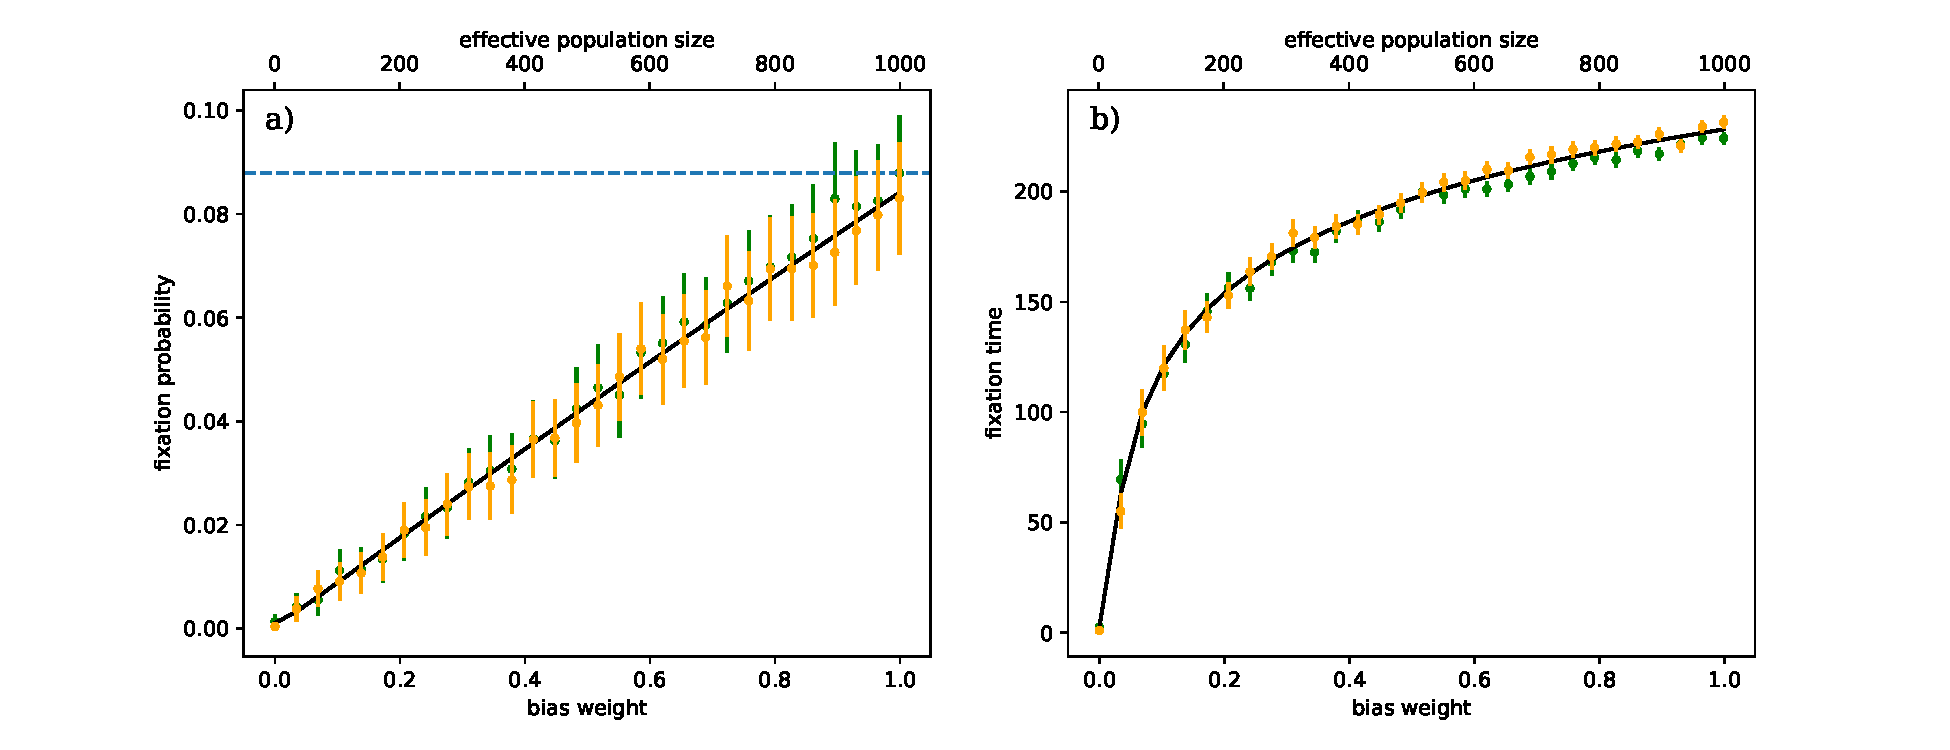
\includegraphics[width=\linewidth]{../figures/binary/kimura_var_alpha.pdf}
  \caption{\textbf{Goodness of fit of Kimura's approximation for varying bias weights.}
  The approximation (black) fits DM simulations results (green) and Wright Fisher simulation results (orange) when using \cref{eq:kimura_p}.
  Fixation probability (a) is limited at approximately $2s$ (blue), like the classic WF model.
  Markers for average values across $5,000$ simulations, error bars for 95\% confidence intervals.
   Here, Population size, $N=1,000$; phenotype values, $\hat{A}=1$, $A=0.7$; success coefficient, $1-\beta=s=0.044$.}
  \label{fig:var_alpha}
\end{figure}

\begin{figure}[h]
    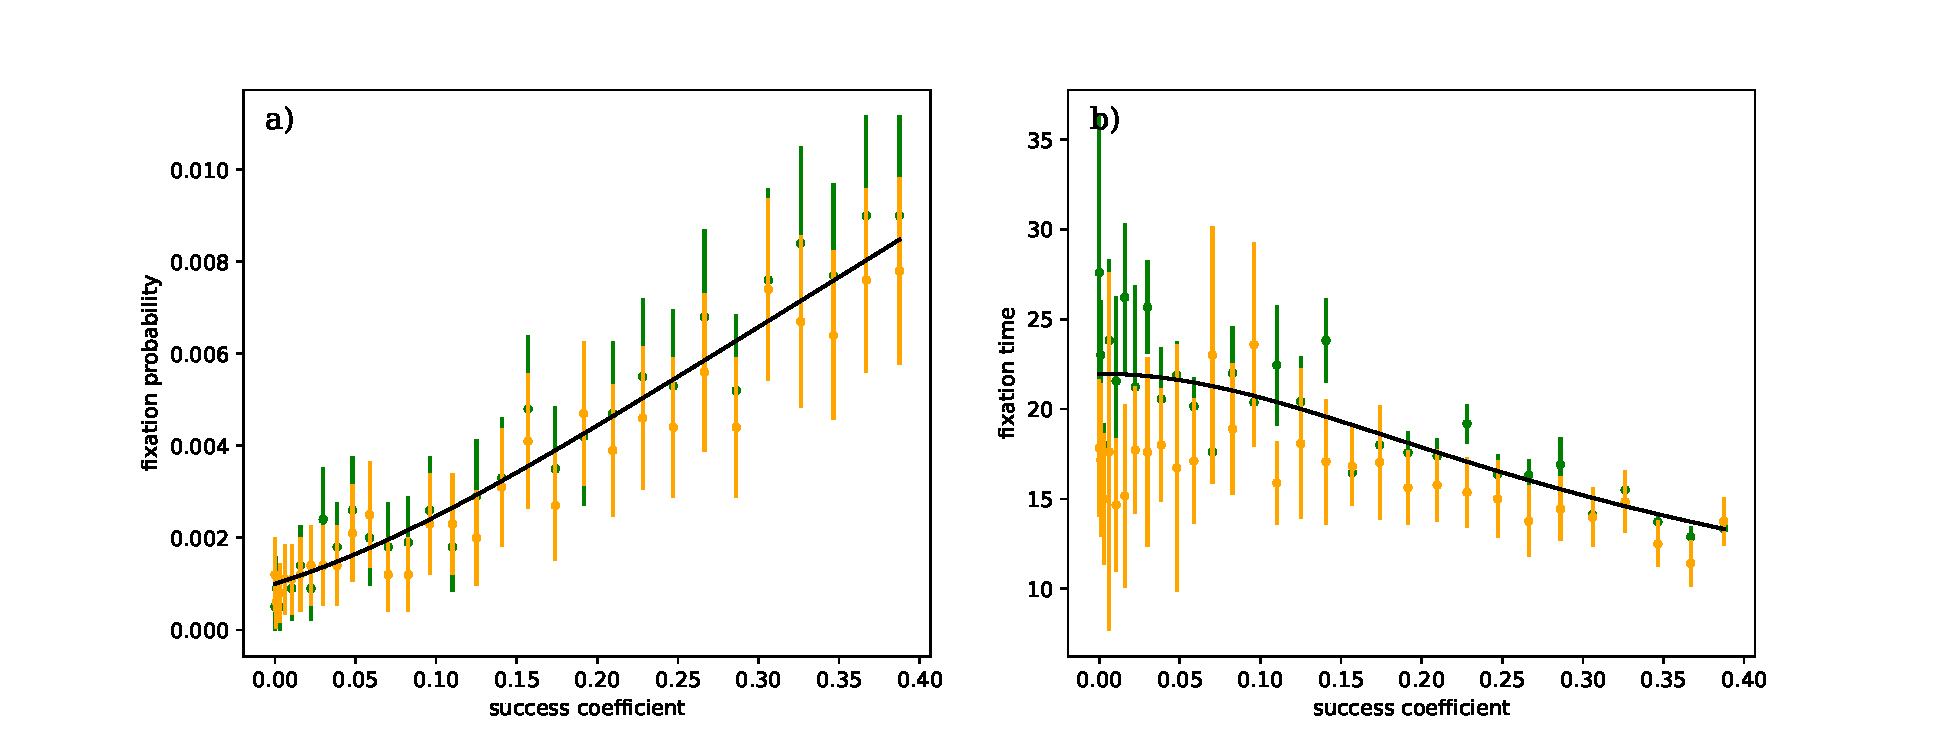
\includegraphics[width=\linewidth]{../figures/binary/kimura_var_beta.pdf}
  \caption{\textbf{Goodness of fit of Kimura's approximation for varying success coefficients.}
   The approximation (black) fits DM simulations results (green) and Wright Fisher simulation results (orange) when using \cref{eq:kimura_p}.
  Markers for average values across $5,000$ simulations, error bars for 75\% confidence intervals.
 Here, Population size, $N=1,000$; phenotype values, $\hat{A}=1$, $A=a\cdot \hat{A}, a \in [0.01,0.99]$; bias weight, $\alpha=0.01$.}
  \label{fig:var_beta}
\end{figure}

After finding good estimations for our model in a constant environment, when the favorable trait is always $\hat{A}$, we want to find an estimation for our model in a changing environment.

For that we will find an expression for the expected and variance of the change in frequency between $t$ generations.
Let $s_t=N(1-\beta_t)$, and $S_n=\sum\limits_{i=1}^n s_i$, where $\beta_t$ is $\beta(A)$ at time/generation $t$.

\begin{result} [Expected difference in frequency in a changing environment]\label{res:ch_expected}
$E[\frac{X_t}{N}-x]\simeq \frac{1}{N}S_tx(1-x)$, where $x$ is the initial frequency of the favorable/invading trait and $X_t$ is the number of individuals with the trait at time $t$.
\end{result}
\begin{result}[Variance of difference in frequency in a changing environment]\label{res:ch_var}
$V(\frac{X_t}{N})\simeq\frac{1}{N_e}tx(1-x)$, where $x$ is the initial frequency of the favorable/invading trait and $X_t$ is the number of individuals with the trait at time $t$.
\end{result}

\begin{proof}
Following the proof of \citet{changeEnv}, we prove by induction. We will prove \cref{res:ch_expected,res:ch_var} together, because the induction assumptions are needed for both.

From \cref{eq:expec_freq} we know that
\begin{equation}\label{eq:ch_1}
\begin{split}
E\left[\frac{X_{t+1}}{N}-\frac{X_t}{N}\bigg|X_t\right] &= \frac{X_t}{N}\left(1-\frac{X_t}{N}\right)(1-\beta_{t+1}) \\
&= \frac{1}{N}\frac{X_t}{N}\left(1-\frac{X_t}{N}\right)s_{t+1}
\end{split}
\end{equation}
Also note that using the definition of $V(y)=E[y^2]-(E[y])^2$
\begin{equation}
\begin{split}
E\left[\frac{X_t}{N}\left(1-\frac{X_t}{N}\right)\right] &= E\left[\frac{X_t}{N}-\left(\frac{X_t}{N}\right)^2\right] \\
&= E\left[\frac{X_t}{N}\right]-E\left[\left(\frac{X_t}{N}\right)^2\right] \\
&= E\left[\frac{X_t}{N}\right] - V\left(\frac{X_t}{N}\right) - \left(E\left[\frac{X_t}{N}\right]\right)^2
\end{split}
\end{equation}

we can now use the induction assumption of $V(\frac{X_t}{N})$ and get
\begin{equation}
\begin{split}
E\left[\frac{X_t}{N}\left(1-\frac{X_t}{N}\right)\right] &\simeq
E\left[\frac{X_t}{N}\right]\left(1-E\left[\frac{X_t}{N}\right]\right)-\frac{1}{N_e}tx(1-x)
\end{split}
\end{equation}
From \cref{eq:ch_1} we know that
\begin{equation}
\begin{split}
E\left[\frac{X_{t+1}}{N}-\frac{X_t}{N}\right] &= \frac{1}{N}s_{t+1}E\left[\frac{X_t}{N}\left(1-\frac{X_t}{N}\right)\right] \\
&\simeq \frac{1}{N}s_{t+1}\left(E\left[\frac{X_t}{N}\right]\left(1-E\left[\frac{X_t}{N}\right]\right) - \frac{1}{N_e}tx(1-x)\right) \\
&\simeq \frac{1}{N}s_{t+1}\cdot E\left[\frac{X_t}{N}\right]\left(1-E\left[\frac{X_t}{N}\right]\right) - \frac{1}{N_e N}s_{t+1}tx(1-x)
\end{split}
\end{equation}
Now we'll omit $O(\frac{1}{Ne\cdot N})$ and get
\begin{equation}\label{eq:ch_2}
E\left[\frac{X_{t+1}}{N}-\frac{X_t}{N}\right] \simeq \frac{1}{N}s_{t+1}\cdot E\left[\frac{X_t}{N}\right]\left(1-E\left[\frac{X_t}{N}\right]\right)
\end{equation}

We'll now look at the induction assumption to see that
\begin{equation}
E\left[\frac{X_t}{N}-x\right]=E\left[\frac{X_t}{N}\right]-E[x]=E\left[\frac{X_t}{N}\right]-x ,
\end{equation}
so using the assumption we get
\begin{equation}
\begin{split}
E\left[\frac{X_t}{N}\right] &\simeq \frac{1}{N} S_t x(1-x)+x \\
1 - E\left[\frac{X_t}{N}\right] &\simeq 1- \frac{1}{N} S_t x(1-x)+x
\end{split}
\end{equation}
we'll use both expressions in \cref{eq:ch_2} and get
\begin{equation}\label{eq:ch_3}
\begin{split}
E\left[\frac{X_{t+1}}{N}-\frac{X_t}{N}\right] &\simeq \frac{1}{N}s_{t+1} \left(\frac{1}{N} S_t x(1-x)+x \right)\left(1- \frac{1}{N} S_t x(1-x)+x \right) \\
&\simeq  \frac{1}{N}s_{t+1}\cdot x(1-x)
\end{split}
\end{equation}
after again omitting $O(\frac{1}{N^2})$ parts of the equation.
To conclude our proof, we see that
\begin{equation}
E\left[\frac{X_{t+1}}{N}-x\right] = E\left[\frac{X_{t+1}}{N}-\frac{X_t}{N}\right] + E\left[\frac{X_t}{N}-x\right]
\end{equation}
so again using the induction assumption, together with \cref{eq:ch_3} we get
\begin{equation}
\begin{split}
E\left[\frac{X_{t+1}}{N}-x\right] &\simeq \frac{1}{N}s_{t+1}\cdot x(1-x) + \frac{1}{N}S_t\cdot x(1-x) \\
& \simeq \frac{1}{N}x(1-x)(S_t + s_{t+1}) \\
& \simeq \frac{1}{N} S_{t+1} x(1-x)
\end{split}
\end{equation}
which proves \cref{res:ch_expected}.

For \cref{res:ch_var}, we'll use a property of variance:
\begin{equation}\label{eq:ch_var}
V\left(\frac{X_{t+1}}{N}\right) = E\left[V\left(\frac{X_{t+1}}{N} \bigg|X_t \right)\right] + V\left(E\left[\frac{X_{t+1}}{N} \bigg|X_t \right]\right)
\end{equation}

using \cref{eq:ch_1} we see that:
\begin{equation}\label{eq:ch_var1}
\begin{split}
E\left[\frac{X_{t+1}}{N} \bigg|X_t \right] - E\left[\frac{X_{t}}{N} \bigg|X_t \right] &= \frac{1}{N}s_{t+1}\frac{X_t}{N}\left(1-\frac{X_t}{N} \right) \\
E\left[\frac{X_{t+1}}{N} \bigg|X_t \right] = \frac{X_t}{N} &+ \frac{1}{N}s_{t+1}\frac{X_t}{N}\left(1-\frac{X_t}{N} \right)
\end{split}
\end{equation}

Using \cref{eq:const_var} we get:
\begin{equation}
V\left(\frac{X_{t+1}}{N} \bigg|X_t \right) = \frac{1}{N_e}\frac{X_t}{N}\left(1-\frac{X_t}{N} \right)
\end{equation}

and using the equation $y'(1-y') \simeq y(1-y)$ on the first part of \cref{eq:ch_var} we get:
\begin{equation}\label{eq:ch_var2}
E\left[V\left(\frac{X_{t+1}}{N} \bigg|X_t \right)\right] = \frac{1}{N_e}E\left[\frac{X_t}{N}\left(1- \frac{X_t}{N}\right) \right] \simeq \frac{1}{N_e} x(1-x)
\end{equation}

and moving on to simplify the second part of \cref{eq:ch_var} using \cref{eq:ch_var1}:
\begin{equation}
V\left(E\left[\frac{X_{t+1}}{N} \bigg|X_t \right]\right) = V\left(\frac{X_t}{N} + \frac{1}{N}s_{t+1}\frac{X_t}{N}\left(1-\frac{X_t}{N} \right) \right)
\end{equation}

and now, because $\frac{X_t}{N}$ is a frequency, i.e $0\leq\frac{X_t}{N}\leq1$, we know that $V\left(\frac{X_t}{N}\left(1-\frac{X_t}{N} \right) \right)\leq\frac{1}{4}$. We therefore see that:
\begin{equation}
V\left(\frac{1}{N}s_{t+1}\frac{X_t}{N}\left(1-\frac{X_t}{N} \right) \right)\leq \frac{1}{4N^2}s^2_{t+1}
\end{equation}
and so it can be ignored.
Combining our equations we get:
\begin{equation}
V\left(E\left[\frac{X_{t+1}}{N} \bigg|X_t \right]\right) = V\left(\frac{X_t}{N}\right) + O\left(\frac{1}{N^2}\right)\simeq V\left(\frac{X_t}{N}\right)
\end{equation}

Using the induction assumption and \cref{eq:ch_var2}:
\begin{equation}
V\left(\frac{X_{t+1}}{N}\right) \simeq \frac{1}{N_e}x(1-x) + \frac{1}{N_e}tx(1-x) \simeq \frac{1}{N_e}x(1-x)(t+1)
\end{equation}
proving \cref{res:ch_var}.
\end{proof}

Following our proof, we can say that after many cycles, we can use a modified version of our fixation probability:
\begin{equation}\label{eq:ch_env}
P_{fix} = \frac{1-e^{-2 \frac{S_n}{n} N_e x}}{1-e^{-2 \frac{S_n}{n} N_e}}
\end{equation}
where $\frac{S_n}{n} = \frac{k-l}{k+l}(1-beta)$, $n=k+l$. Put into words, we use the average selection coefficient of a cycle ($k+l$) as the selection coefficient in our original equation.
In our proof we showed that the expected change in frequency and variance is only manifested in the selection coefficient $S_n$, and that we can use those modified equation as a base for Kimura's equation.

\begin{figure}[h]
    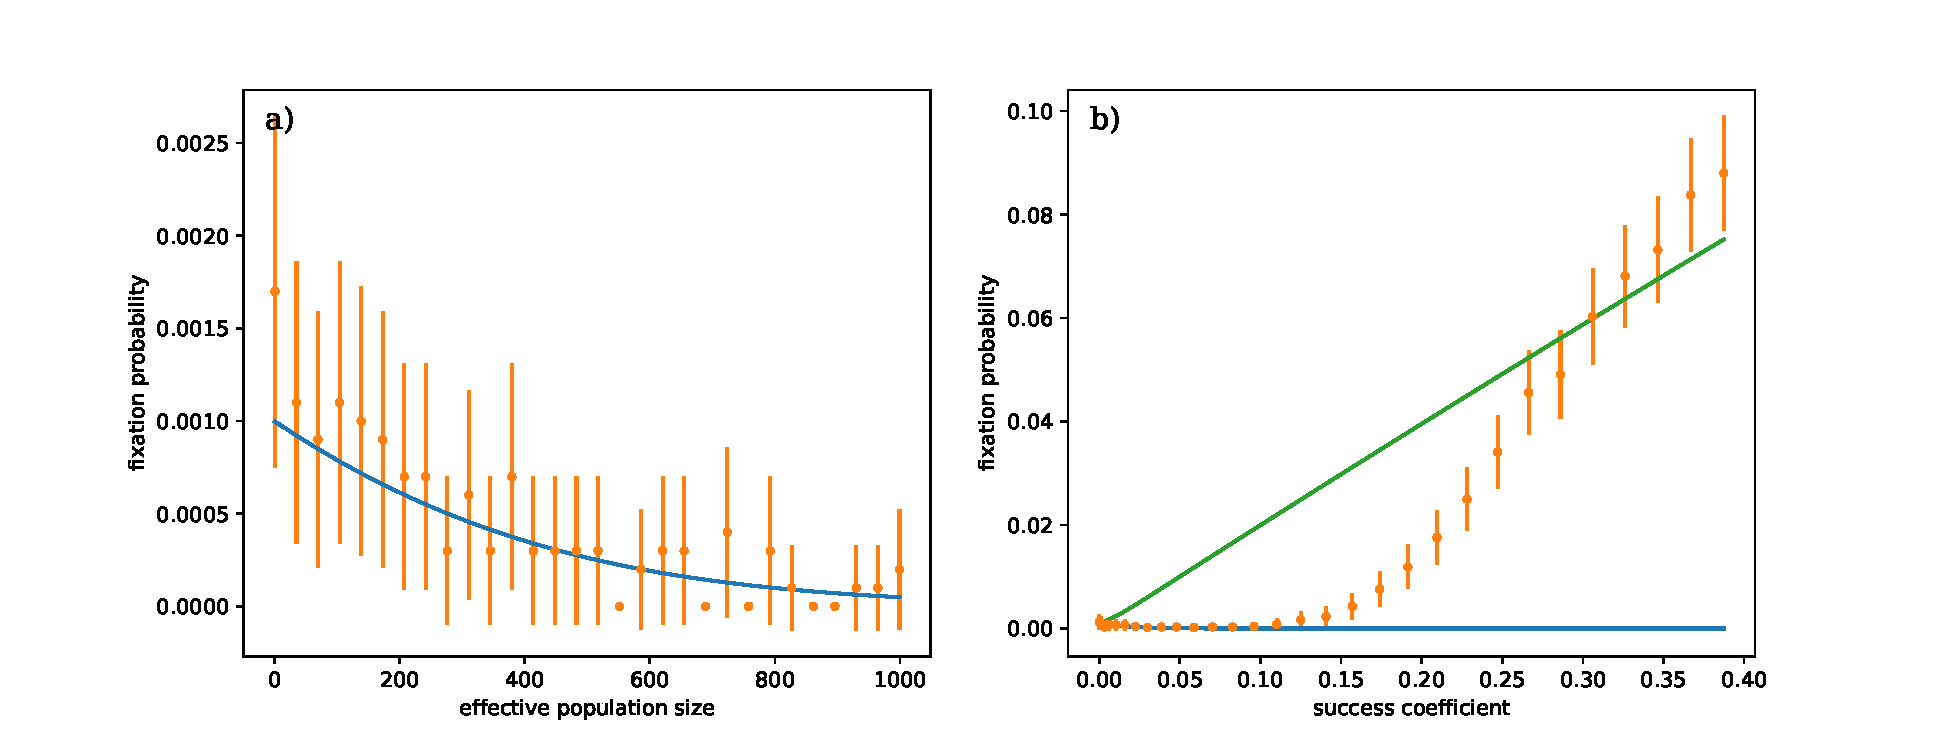
\includegraphics[width=\linewidth]{../figures/changed_env/ch_env_var.pdf}
  \caption{\textbf{Robustness of approximation in a changing environment to varying success coefficient and success bias weight.}
 Markers for average values across $10,000$ simulations, error bars for (a) are 75\% confidence intervals, and 95\% for (b).
The approximation (blue) given by \cref{eq:ch_env} fits simulation results (orange) well when the effective population size varies (a).
On (b) we see that for high values of success bias ($s>0.1$) will distance the simulations from the changing environment expected values. Very high values ($s>0.35$) will even deviate from the constant environment expected values (green) given by \cref{eq:kimura_p}. This is expected because Kimura's approximation are only viable for low selection coefficient values.
  Here, population size, $N=1,000$; phenotype values, $\hat{A}=1$, $A=0.9$; \textbf{(a)} success bias/selection coefficient is: $1-\beta=s=0.005$, \textbf{(b)} success bias weight is: $\alpha=0.1$. 
  }
  \label{fig:ch_env_alpha_beta}
\end{figure}

We validate our results using simulations.
We find that $\alpha$ does not have a significant effect on the approximations (\cref{fig:ch_env_alpha_beta}).
However, $\beta$ does. 

We suspect that when $1-\beta$ is too large, there won't be many cycles in the simulations. This might happen if either the population reaches a high frequency of the fitter phenotype after only a few cycles, or the fitter phenotype get extinct very quickly. 
For the very high $1-\beta$ values (0.35 and above), the fixation probability exceeds even the constant environment approximation (which is the upper limit), but it's to be expected, because Kimura's equations are only appropriate for weak fitness (i.e., low selection coefficients, $s$).

\begin{figure}[h]
    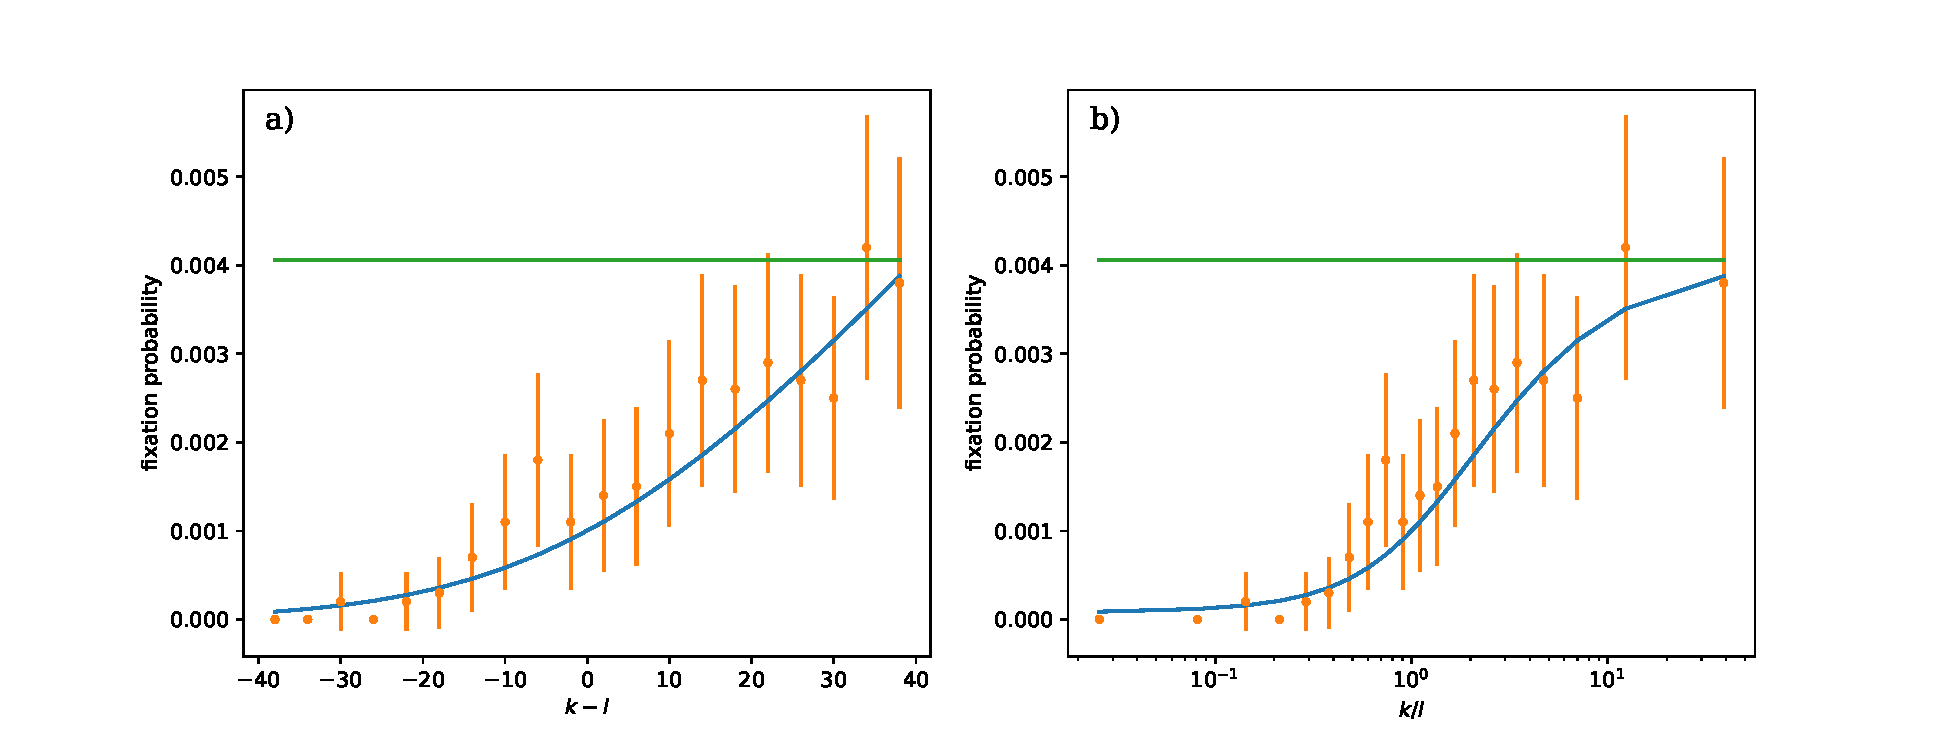
\includegraphics[width=\linewidth]{../figures/changed_env/ch_env_var_k_l.pdf}
  \caption{\textbf{Robustness of approximation in a changing environment to varying sizes of the cycles.} 
Markers for average values across $10,000$ simulations, error bars are 95\% confidence intervals.
The approximation (blue) fits the simulations (orange) well for different sizes of the changing environment cycle, where $k$ is the number of generations where the bias is advantageous, and $l$ are the generations it is disadvantageous.
   When $k<l$ the approximation is good. When $k>l$, the approximation and the simulations are both very close to the constant environment approximation (green). 
 Here, population size, $N=1,000$; phenotype values, $\hat{A}=1$, $A=0.8$; success coefficient, $1-\beta=s=0.02$; success bias weight, $\alpha=0.1$.}
  \label{fig:ch_env_k_l}
\end{figure}

We also examined the effect of different choices of $k$ and $l$ while keeping a constant total cycle length, $n=k+l=40$.
We found that larger $k$-to-$l$ ratio increases the agreement between the changing environment equation and the original estimation of the constant environment. 
When using higher values of $n$, the agreement between the approximation and simulation results is weaker.
This is because our approximation is more precise when more cycles occur.
When $n$ is high, the cycles are longer. When the cycles are long, the settings are similar to a constant environment equation, and fixation/extinction is more likely to happen. This means there will be less cycles, which lowers our approximation accuracy.

%%%%%%%%%%%%%%%%%%%%%%%%%%%%%%%%%%%%%%%%%%%%%%%%%%%%%%
\subsection*{Adaptive success-bias weight}

We ran simulations of the role-model choice process during a single generation in which every copier evaluates its own optimal $\alpha$ value. This is the $\alpha$ value that minimizes the mean error in estimation. % TODO estimation of what?
This is computed by minimizing the mean difference between the estimated value of every role-model and the ideal trait value $\hat{A}$. % TODO write the explicit equation

We see in \cref{fig:influence_advantage,fig:const_influence} a comparison between a model where every copier chooses its ideal success bias weight $\alpha_{ij}$, and when $\alpha$ is a constant homogeneous value.
We find that when copiers adapt their success-bias weight, their success-bias weight decreases with the number of copiers that have already chose a role-model~(\cref{fig:influence_advantage}a).
Moreover, their estimation error is much lower compared to a constant success-bias weight, which gives roughly the same high estimation error to all copiers (compare \cref{fig:influence_advantage}b and c): the estimation error converges to $0.046$ whereas a constant weight gives values $>0.74$ in this example.


\begin{figure}[b!]
    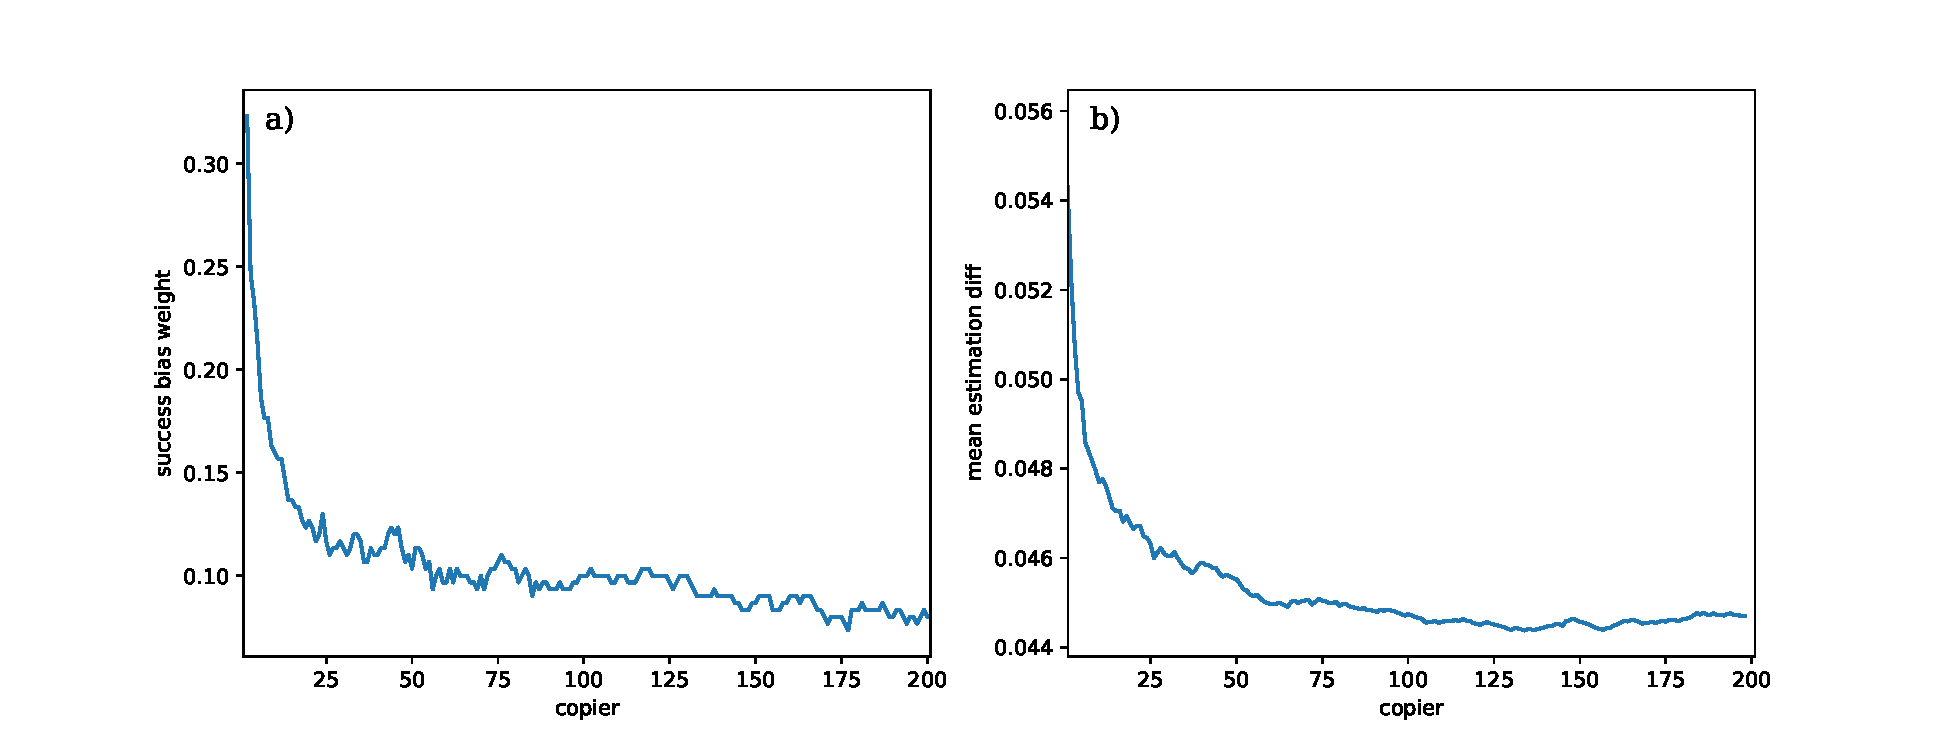
\includegraphics[width=\linewidth]{../figures/influence_advantage/choose_bias.pdf}
    % TODO
    % fonts too small
    % capital letters in labels
    % add "alpha" to ylabel in panel a
    % "mean estimation error" in y label of panel b
	% can you maybe add two more lines with different colors on the same plots for other parameters choices? say larger pop size or larger error?
  \caption{
  \textbf{Advantage of an adaptive success-bias weight.}
  Both success-bias weight $\alpha$ (\textbf{a}) and estimation error (\textbf{b}) 
   decrease during the role-model choosing process, demonstrating that influence is becomes more advantageous as more copiers have made their choice.
   Here, population size $N=200$, estimation error is normally distributed $e \sim N(0,\eta^2)$, standard deviation $\eta=0.0005$, plots are average of $300$ simulations.}	
  \label{fig:influence_advantage}
\end{figure}

\begin{figure}[h]
    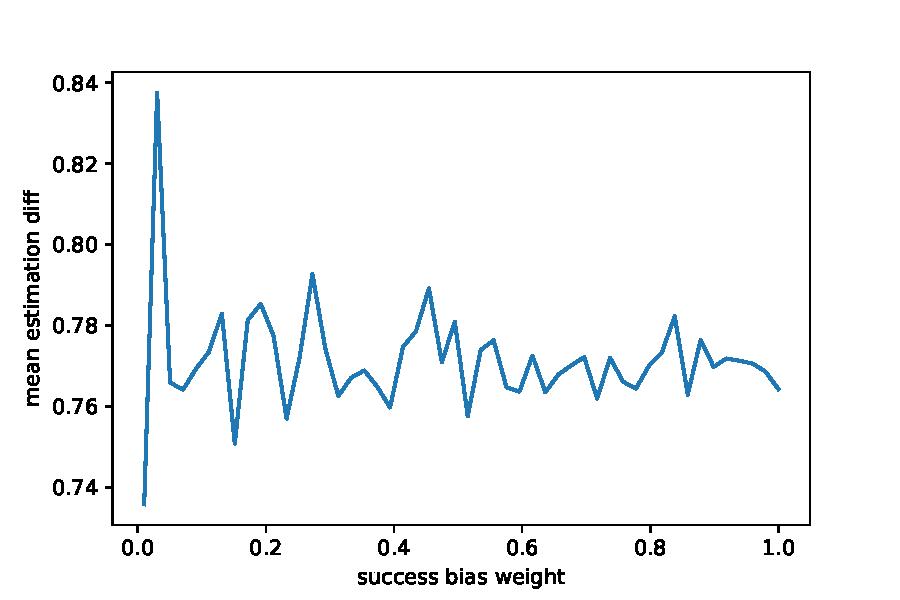
\includegraphics[width=\linewidth]{../figures/influence_advantage/const_bias.pdf}
    % TODO 
    % merge with previous plot
  \caption{
  \textbf{Estimation error when using constant success bias weight.}
  The mean estimation error doesn't have any significant improvement relative to when every copier chooses a bias for himself.
  The minimum error is no less than $0.74$, while the mean error of the model where $\alpha$ is chosen is $0.06$, converging to $0.046$, which is a factor of $10$ less than the constant $\alpha$ model, showing the clear advantage of choosing $\alpha$.
  Here, population size $N=200$, estimation error is normally distributed $e \sim N(0,\eta^2)$, standard deviation $\eta=0.0005$, plots are average of $300$ simulations.}	
  \label{fig:const_influence}
\end{figure}

%%%%%%%%%%%%%%%%%%%%%%%%%%%%%%%%%%%%%%%%%%%%%%%%%%%%%%
\section*{Discussion}
\paragraph{Summary.}
During cultural transmission, cultural traits such as attitudes, values, beliefs, and behavioral patterns are transmitted between individuals, for example via copying and social learning.
Some cultural traits or cultural role-models may be more likely to be copied due to transmission biases. 
A common one is success bias, in which copiers are more likely to copy a successful role-model. Many models assume that success can be accurately estimated.
However, it has been suggested \citep{complexityPaper} that because estimating success is hard, a more common bias is \textit{prestige bias}---a bias towards role-models perceived to be successful, portrayed by other traits or means.

Inspired by a model by \citet{evolutionBook}, we developed a cultural-evolution model with prestige bias, which included both success and influence biases, where the latter is a bias towards role-models with many copiers.
As shown in \cref{fig:influence_advantage}, given the option to choose the ratio of success and influence, copiers will minimize their estimation error, hence will copy the traits that are closer to the ideal phenotype. We see that throughout the choosing process, the estimation error decreases, and the success bias rate also decreases. This suggests that the later a copier gets to choose, the less he should rely on his own estimation, and more on previous choices.
This behavior fits the intuitive thought - the more information you have, using others as an information source, the more informative your choice can be, therefore minimizing the distance from your choice of trait to the ideal one.

In addition, we see that the process of choosing itself is necessary, and when using a constant ratio ($\alpha$), the mean estimation error in the population is greater by a factor of $10$, even when using the $\alpha$ the population converged to when being able to choose it (\cref{fig:const_influence}).
After we showing that choosing one's success bias weight is beneficial to the copier, we continued to create our models- continuous and dichotomous, that incorporated both success and influence. However, running simulations for a nested iterative model is costly, and analyzing such model mathematically is very hard. We therefor found approximations for the role-model choice process: the generalized binomial distribution (\cref{res:GBD}) and the Dirichlet-Multinomial distribution (\cref{cor:dirichlet}).
To use approximate our model with the GBD distribution, we must assume homogeneous estimation error, $e$, and homogeneous success bias weight, $\alpha$. Both assumptions are necessary to this approximation, because it requires all copiers to be identical (order of copiers must not be a factor).
For the DM approximation we can relax the assumption for $\alpha$, and allow a varying $\alpha_j$ for each role-model $j$. This means that a copier is still not able to choose a success bias weight for itself, and instead it is a characteristic of the role-model only.
Using the DM approximation, because it is easier to analyze, we found equivalents for Kimura's equations, for our dichotomous model.
Following \cref{res:selection_coef,res:effective_population} we found an approximation for the fixation probability of the ideal trait, and an approximation for the time of fixation. These approximations hold only when the equivalent for the selection coefficient, in our model $1-\beta(A)$, is low (0.4 or lower). We also discovered that changing the success bias weight doesn't hurt the goodness of the approximations, and only affects the effective population size $N_e$.
Once we found the equations for a constant environment, we moved on to a cyclic changing environment.
Based on \cref{res:ch_expected,res:ch_var}, we found the approximations for the fixation probability and time to fixation.
We discovered that as in the constant environment, the effective population size doesn't affect the goodness of fit of the approximation. The success coefficient however, must be even lower than before for the approximation to fit. When the success coefficient is higher than 0.15, the simulation results were located above the changing environment approximation, and below the constant environment approximation. We believe the reason is the structure of the cycle.
Our proof and approximation in the changing environment are for a large amount of cycles, and when the success coefficient is too high, there might be very few cycles. Either the ideal trait is copied by enough copiers so that the influence is sufficient to negate the success bias when the cycle changes (and the beneficial trait becomes the maladaptive), or the opposite happens, and the ideal trait gets extinct before there were enough copiers that copied it.
We then tried to change the ratio between the number of cycles where $\hat{A}$ is beneficial and maladaptive. We showed that the approximation fits well regardless of the ratio, but when the ratio of adaptive generations to maladaptive ones is very high, it is very similar to a constant environment model.

\paragraph{Prestige in the literature.}

According to \citet{animal_leadership}, there are two main approaches to group decision-making in nature: leadership and consensus.
Leaders may lead the group when traveling, decide on a nesting site, or choose foraging patches. They found that leadership is mostly observed when there are a lot of connections in the social network of the group, and when there are individuals that present leadership behavior.
Leaders would usually be high-ranking members of the group: elders, individuals with many kin relations, or individuals possessing other dominant traits.
When no individual posseses such traits, or when there are not enough connections and relations in the social network, decisions are more likely to be made by consensus.
Leaders may carry selection costs, e.g. due to higher predation risk, poisoning when exploring new foraging patches.
In some cases, the leader may be the hungriest or the weakest individual, while the others would prefer to follow the leader and minimizing their risks and costs.
However, leadership may also carry selection benefits. For example, given the route to the foraging site was successful, the leader and his closest followers would gain most or the best of the food, whereas in consensus decision making, the food would be shared more equally. Or, sexual selection may also provide a selection benefit advantage to leaders, who might gain more sexual partners due to their leadership of the group. \citet{animal_leadership} describe benefits for the closest associates of a dominant baboon, such as protection from predators. 
In some species, like the females of \textit{Eulemur fulvus rufus} (Red lemur), leaders may arise due to nutritional needs, and not due to possessing superior traits \citep{lemurs}.

In humans, leadership also has its costs and benefits. Leaders can make decisions that would most benefit them and their closest followers, while still maintaining group cohesion. However, wrong decision making that harms the group could result in harm.

In modern society humans strive for the prestigious positions, as they may reap rewards greater than the risk and costs to achieve them, or due to individual personality and pressure/education from the family.

\citet{dual_leadership} suggest a different view of leadership. They note that most discussions assume there is one type of leadership, as seen above, and so they differ in their definitions. \citet{dual_leadership} suggest a way to solve said contradiction by defining two types of leaderships: prestige-based and dominance-based.
They present classical views of leaderships by Confucius and Machiavelli. Confucius views leaders as role-models who exercise influence through possessing superior knowledge, skills,
and (outstanding) personal qualities. This description is very similar to success bias in our model. 
By contrast, Machiavelli views leaders as rulers who exercise influence by imposing costs through (the threat of) punishment and violence.
They say that these two opposing views are both partially supported by the available evidence but each one on its own offers an incomplete view into the complex and dynamic processes of leadership. 
Our model does not reflect these leadership styles, but several adjustments could be made in order to match it, such as assuming there is a correlation between phenotype to leadership style. 
The emerging cultural-evolutionary dynamics and their dependence on the costs and benefits are intriguing.

\citet{prestige_evolution} support said claim that there are two types of leadership, and also define the two as prestige based and dominance based leadership types.
By their definition, the latter is defined by acquiring social status by using aggression, intimidation and violence. It is also more common than prestige in non humans. Their definition of prestige is somewhat synonymous with ours. According to their manuscript, prestige is composed both of estimation in the eyes of people (our success trait) and commanding position in people's minds, i.e number of copiers people think they have, which they define as \textit{influence} (similar to our definition for influence).
In their paper, they show that prestige evolved from natural selection, as an efficient process to extract reproductive benefit from the flow of socially transmitted information. Simply put, prestige is a natural step where social learning exists, due to saving costs of individual learning.
It could be interesting in the future to expand our model using this idea: observing the copier trait of \textit{evaluation}, rather than only observing the evolution of the trait copied.
\citet{prestige_evolution} suggest that the most skilled role-models will, on average, end up with most copiers. Their research, definitions and results, is consistent with ours.

Furthermore, according to \citet{no_replication}, the process of cultural evolution doesn't require replication of representations.
They base their assumption on three claims - mental representations are non-discrete, cultural transmission is highly inaccurate, and mental representations are not replicated, but rather are 'reconstructed' through an inferential process that is strongly affected by cognitive 'attractors.' In their paper they describe three different models to support their points.
We see a high similarity between their model and ours. Like them, we treat the cultural trait as non-discrete (in the main model, before simplifying it to dichotomous in order to analyze it). We also assume error in estimation, which the copiers aren't really replicating their role-models, but rather reconstructing them to create a different trait, which is their representation of the role-model's trait. In addition, the inferential process that they describe as strongly affected by cognitive attractors match our influence bias, resulting in a very similar base assumptions in our models.

So far we presented the theory behind prestige, and it's appearance in nature. The following will show the appearances of prestige biases in humans, and in recent times.

\citet{prestige_cultural_learning}, for example, tested the existence of prestige in young children. \citet{prestige_cultural_learning} report the first direct tests in children that suggest the existence of \textit{prestige bias}, a tendency to learn from individuals to whom others have preferentially attended, learned or deferred.
Their definition of prestige is similar to our \textit{influence bias}, and brings concrete proof of its existence and effects. Their study showed that the odds of 3-4 years-old children learning from an adult model to whom bystanders had previously preferentially attended for 10 seconds were over twice those of their learning from a model whom bystanders ignored.
In addition to this first study, they also discovered prestige effects are domain-sensitive. They saw that prestigious models were listened to by most when demonstrating artifact-use, but not as much as when presenting food preferences. It lead \citet{prestige_cultural_learning} to believe that when the trait is costly to learn individually, prestige will have a higher effect. It would be interesting to include costs in our model to try and observe these effects and their dynamics in the simulations of a larger population than this study.

\citet{fijian_social_bias} researched Fijian villages, looking for evidence of social learning biases and their origins. They mention that:
\begin{quote}
evolutionary theorists propose that natural selection has favored the emergence of psychological biases for learning from those individuals most likely to possess adaptive information.
\end{quote}
Their goal is to bridge from the laboratory to the field by examining if and how these biases emerge in a small-scale society.
During their research they found that:
\begin{quote}
Fijian villagers (ages 10 and up) are biased to learn from others perceived as more successful/knowledgeable, both within and across domains (prestige effects).
\end{quote}
Their research shows promising evidence for our prestige model, suggesting that copying from others who are \textit{perceived} as successful, rather than actually are successful. In their paper, they show that the social networks representing copier-role-model relationships are centralized, suggesting:
\begin{quote}
This degree of centralization is consistent with the prediction that people substantially share notions about who is a good cultural model (network centrality), but that individuals’ model selections are influenced by multiple factors.
\end{quote}
We see here support for both our trait and our influence bias in their data.

Aside from children's learning biases and small villages in a relatively primitive population, we can see prestige in more advanced domains as well, like western medicine.\citet{medical_prestige} present a specific and important effect of prestige - its significance for medical specialties and diseases.
They examined literature from 1950 to 2005 regarding the effects of prestige on medicinal practices. They discovered that active, specialized, biomedical, and high-technological types of medicine on organs in the upper part of the bodies of young and middle-aged people were accorded high levels of prestige, while medicine with opposite characteristics had low levels of prestige. They have concluded that such differences in prestige bear consequences for actual priority setting in healthcare systems. They discovered that surgery counts as the most prestigious specialty, while psychiatry is the less prestigious. In addition, doctors tend to rank practices that require more time to master as more prestigious, while other procedures that are considered \textit{easier} are less prestigious. Simply put, they found that the advance in technology and research was in accordance with the prestige rankings.
This means that there may be very important practices that are neglected due to the prestige bias.

As we seen so far, prestige can explain many behaviors and evolution of cultural traits. It is a tool to cheaply estimate and acquire knowledge, which helps an individual to survive and breed. However, it is not always the case, and there could be negative repercussions to this bias, such as invasion of maladaptive traits.

\citet{best_of_k} mention that social learning not only takes the form of random copying of other individuals, but also involves learners’ choice of what to learn and from whom to learn. They suggest a best-of-K model where an individual samples k role-models and choose the one he deems most "successful". They mentioned that a previous mathematical analysis has shown that it may sometimes result in maladaptive cultural evolution when the payoffs associated with cultural variants vary stochastically. In such a case, learners may be selectively disfavored and in the long run replaced by unbiased learners, who simply copy someone chosen at random. They develop new mathematical models that are simpler and mathematically tractable. They found that best-of-k learning, unlike unbiased learning, can facilitate the invasion of an on average inferior variant that sometimes gives a very high payoff. Our model, which includes influence bias, is consistent with that claim. When a maladaptive trait is "piggybacking" a role-model with high influence, said trait could spread in the population, as mentioned. In addition, they show that best-of-k learning can be stable against invasion by unbiased learning if social learning is sometimes combined with individual learning. Our model is based on copying based learning only, but it could be interesting to combine it with individual learning and see how it affects the dynamics of the population.

We discussed prestige in depth, and provided several proofs for its existence in nature, humans, and even medicine. We saw it could aid invasion of maladaptive traits, or neglect of important medicinal specialities. But, it can also accelerate reversal of harmful traditions.
Harmful traditions can be child marriage, open defecation, and domestic violence, to name a few. 
\citet{harmful_traditions} suggest a mechanism called \textit{spillover}. By their definition, a spillover is when an intervention affect a large enough group in a target population, so that others not included in the intervention starts changing their behavior as well. In their research, they found that there are individuals who act as \textit{agents}, who are often looked upon, and therefore they are ideal targets for interventions. This is the same concept as our role-models, where a more prestigious individual will be copied more, therefore spreading his trait wider in the population. Their research support therefore in our assumption that there are social biases, conformist influence specifically. They also suggest a way to use this phenomena to change existing traditions in a population. It is very clear however, that just as it can be used to end harmful traditions, the same agents could be used for any negative way that comes to mind.

Up until now, we showed that cultural transmission is a process that manifests in many species, with emphasis on humans. We also displayed similarities between this process and genetic transmission, while presenting differences between them, specifically selective biases such as influence and prestige. We also presented examples of good and bad usages of such biases. All of these are mainly presented as a parallel process to the natural selection process in regards to physical anatomy, or at least have an indirect effect on it. \citet{collective_brains} offer a take on prestige as a factor of human physical evolution directly. They present a concept called \textit{cultural brains} | brains that evolved primarily for the acquisition of adaptive knowledge.
They build on the hypothesis of \citet{social_brains} that shows that larger, more complex brains can store and manage more information and in turn, this information can support the costs of a larger brain.
\citet{collective_brains} built a model that predicts a strong relationship between brain size and group size, because group size also provides access to more adaptive knowledge. They later present their \textit{cumulative cultural brain} hypothesis, an approach which proposes that human brains have evolved with an ability and proclivity for selective, high fidelity social learning. As part of this process, there are a variety of strategies and biases that have evolved to hone in on the most adaptive knowledge. These strategies and biases include direct and indirect cues of the popularity of cultural traits (e.g. success and prestige biases).
In short, they suggest that some of the reasons for the extreme increase in brain size in humans, are the ability to "cheaply" acquire adaptive knowledge, i.e transmission biases, such as prestige.

\paragraph{Further work.}
In this paper we described several models and processes, analyzed them, and discovered some interesting approximations and results. But even though, there's much more to research in the direction we took, which can help us better model, understand, and maybe even predict, human behavior, specifically in this era where social media is very accessible and informative.
Specifically, a deeper analysis of the first model, where every copier chooses its $\alpha$, is preferred. It would be interesting to see the if the mean error value and the $\alpha$ are converging to specific values, and what they depend on.
Following that, it is possible to relax some assumptions we took in our main model in order to find approximations for it - like homogeneous estimation error and success bias weight.
Lastly, it would be interesting to analyze the continuous model, instead of its dichotomous version. As we've discussed it is probably a much more accurate model of cultural evolution.

{\small
\section*{Acknowledgements}
We thank Marcus Feldman, Martin Pontz, and Tal Simon for discussions and comments.
This work was supported in part by 
the Israel Science Foundation (YR 552/19),
Minerva Stiftung Center for Lab Evolution (YR),
and 
John Templeton Foundation (YR 61809).
}

\section*{References}
\nolinenumbers
\bibliography{refs}
%\bibliographystyle{agsm}
\bibliographystyle{apalike}
\end{document}
